\documentclass[journal]{IEEEtran}

\usepackage{graphicx}
\usepackage{amsmath}
\usepackage{amssymb}
\usepackage{cite}
\usepackage{booktabs}
\usepackage{multirow}
\usepackage{array}
\usepackage{url}
\usepackage{balance}
\usepackage[hidelinks]{hyperref}

\graphicspath{{figures/}}

\title{
Robust Cross-Domain Climate Scene Classification Across UAV and
Satellite Imagery: Generalization Analysis, External Validation,
and Contextual Shortcut Discovery
}

% TODO: replace with final authors
\author{
Author 1,
Author 2
}

\begin{document}
\raggedbottom

\maketitle

\begin{abstract}
Climate-related aerial scene classification is commonly evaluated
using random train--test splits, although such protocols may
overestimate robustness when images originate from heterogeneous UAV,
satellite, aerial, and aggregated sources. This study investigates
cross-source generalization for three-class classification of Flooded,
Desert, and Neither scenes using a 6,334-image climate dataset.

A custom convolutional neural network and an ImageNet-pretrained
MobileNetV2 pipeline are evaluated under mixed and source-disjoint
protocols, followed by three-seed experiments with conservative
domain-generalization augmentation and Representation
Self-Challenging. External UAV validation is performed using FloodNet.

The MobileNetV2 pipeline achieves a mixed-split Macro-F1 of 0.9775,
but decreases to 0.5274 on the most challenging source-disjoint split.
Across three seeds on this split, ERM obtains
$0.4988\pm0.0259$ Macro-F1, while DG-AUG-V2 and RSC obtain
$0.4831\pm0.0443$ and $0.4883\pm0.0329$, respectively.

External FloodNet evaluation reveals a persistent asymmetric failure:
Flooded recall remains high while Neither recall is substantially
lower. Among 347 external Neither scenes, 178 are predicted as
Flooded by all nine frozen models. Grad-CAM and a post-hoc analysis
of official FloodNet segmentation masks further show that consensus
false-flood scenes contain substantially more ordinary water and
non-flooded road context than consensus-correct Neither scenes.

These findings demonstrate that high mixed-split performance does not
guarantee cross-source robustness and are consistent with reliance on
flood-associated contextual cues rather than a complete semantic
distinction between ordinary water and true inundation.
\end{abstract}

\begin{IEEEkeywords}
Deep learning,
remote sensing,
UAV imagery,
satellite imagery,
domain shift,
domain generalization,
flood classification,
transfer learning,
Grad-CAM,
cross-source generalization.
\end{IEEEkeywords}

\section{Introduction}
\label{sec:introduction}

Flooding and desertification are visible manifestations of
environmental stress that can affect transportation, infrastructure,
agriculture, ecosystems, and human settlements. Aerial and
remote-sensing imagery provides an efficient mechanism for monitoring
large geographic regions; however, automatic scene classification
remains difficult when imagery is collected from heterogeneous
platforms, locations, resolutions, and source datasets.

Deep convolutional neural networks can achieve high classification
accuracy when training and test images are sampled from similar
distributions. Such performance may not reflect deployment robustness,
particularly when images from the same source characteristics are
present in both training and test partitions.

This study therefore treats source-aware evaluation and domain shift
as central components of climate-scene classification. The task is
three-class classification of aerial images into \emph{Flooded},
\emph{Desert}, and \emph{Neither}. The primary dataset contains
6,334 images assembled from multiple underlying sources.

The investigation addresses the following research questions:

\begin{itemize}
    \item \textbf{RQ1:} How much does performance change between
    conventional mixed evaluation and source-disjoint evaluation?

    \item \textbf{RQ2:} How does a MobileNetV2 ImageNet
    transfer-learning pipeline compare with a custom CNN under
    cross-source testing?

    \item \textbf{RQ3:} Do conservative domain-generalization
    augmentation and Representation Self-Challenging improve
    robustness consistently across random seeds?

    \item \textbf{RQ4:} Do the observed failure patterns persist on an
    independent external UAV dataset?

    \item \textbf{RQ5:} Which visual and scene-composition cues are
    associated with systematic external false-flood predictions?
\end{itemize}

The main contributions of this work are:

\begin{enumerate}
    \item high-confidence per-image reconstruction of source
    provenance for the 6,334-image climate dataset;

    \item mixed and source-disjoint evaluation protocols designed to
    expose cross-source generalization failure;

    \item multi-seed comparison of ERM, DG-AUG-V2, and RSC;

    \item external UAV validation using FloodNet with leakage
    screening;

    \item frozen Grad-CAM analysis of correct and systematic
    false-flood predictions; and

    \item post-hoc pixel-level segmentation analysis connecting
    consensus false-flood predictions with ordinary water,
    non-flooded roads, and heterogeneous scene composition.
\end{enumerate}

% TODO: add verified literature citations here.

\section{Related Work}
\label{sec:related}

\subsection{Aerial Disaster and Environmental Classification}

% TODO:
% Flood classification
% Disaster scene classification
% Desertification
% Environmental monitoring
% UAV vs satellite imagery

\subsection{Remote-Sensing Scene Classification}

% TODO:
% CNNs
% Transfer learning
% Pretrained backbones
% Data augmentation
% Evaluation metrics

\subsection{Domain Shift and Cross-Domain Generalization}

% TODO:
% Sensor/platform shift
% Geographic shift
% UAV vs satellite shift
% Domain generalization
% MixStyle
% RSC
% augmentation methods

\subsection{Explainability and Shortcut Learning}

% TODO:
% Grad-CAM
% shortcut learning
% spurious correlations
% contextual bias
% limitations of saliency maps

\subsection{Research Gap}

Existing studies frequently report strong classification performance
under random or within-dataset partitions, but fewer evaluate whether
performance remains stable when complete image sources are withheld.
Independent external validation and quantitative analysis of the scene
characteristics associated with cross-domain failure are also limited.

This study addresses these gaps by combining provenance-aware
evaluation, source-disjoint testing, multi-seed experiments, external
UAV validation, Grad-CAM, and official pixel-level segmentation masks.

\section{Methodology}
\label{sec:methodology}

\subsection{Primary Climate-Scene Dataset and Provenance Reconstruction}

The primary dataset contains 6,334 aerial and remote-sensing images
assigned to three semantic classes: 1,931 \emph{Desert}, 2,338
\emph{Flooded}, and 2,065 \emph{Neither}. The dataset is a heterogeneous
collection assembled from multiple underlying image sources rather than
a single controlled acquisition campaign. Consequently, images belonging
to the same semantic class can differ substantially in acquisition
platform, geographic context, spatial resolution, visual style, and
surrounding scene composition.

To support source-aware evaluation, image-level provenance was
reconstructed for the complete dataset. Eight source groups were
identified, and every image was assigned to one source group with no
unresolved records. This reconstruction is essential because conventional
random splitting can place visually related images originating from the
same source family into both training and test partitions. In contrast,
source-disjoint evaluation can hold entire source groups out of model
development.

The source labels are interpreted as provenance groups rather than
perfectly controlled imaging modalities. Source identity, semantic class,
sensor characteristics, acquisition conditions, and platform are partially
entangled within the assembled dataset. Therefore, the source-disjoint
experiments are treated as composite source-distribution shifts and not
as pure causal UAV-versus-satellite modality experiments.

\subsection{Input Processing and Baseline Augmentation}

All models receive RGB inputs resized to \(224\times224\) pixels. Images
are converted to floating-point values in the interval \([0,1]\). The
class-index mapping is fixed throughout all experiments as

\[
[\text{Desert},\text{Flooded},\text{Neither}]
\rightarrow
[0,1,2].
\]

Augmentation is applied only to the training partition. Validation,
internal test, and external test images are not randomly augmented. The
baseline augmentation pipeline consists of horizontal-and-vertical random
flipping, random rotation with factor \(0.08\), random zoom with factor
\(0.10\), and random contrast with factor \(0.10\). The same baseline
augmentation family is used for CustomCNN\_V1 and the MobileNetV2 ERM
baseline so that architectural comparisons are not confounded by different
standard augmentation policies.

Random seeds are explicitly controlled. The principal baseline
configuration uses seed 42, and TensorFlow deterministic operations are
enabled where supported. Training batches contain 16 images.

\subsection{CustomCNN\_V1 Baseline}

A compact convolutional network, denoted CustomCNN\_V1, is trained from
scratch to provide a non-pretrained reference model. Its purpose is not to
maximize architectural complexity but to establish how far a comparatively
small task-specific CNN can generalize when no external representation
pretraining is used.

The network contains three convolutional feature-extraction blocks. The
first block applies a \(3\times3\) convolution with 32 filters and
``same'' padding, followed by Batch Normalization, ReLU activation, and
max pooling. The second block repeats the same structure with 64 filters,
and the third block uses 128 filters:

\[
32 \rightarrow 64 \rightarrow 128.
\]

After the final pooling operation, Global Average Pooling converts the
spatial feature tensor into a fixed-length representation. This
representation is passed to a fully connected layer with 128 ReLU units,
followed by dropout with probability \(0.40\). The classifier terminates
in a three-unit softmax layer corresponding to Desert, Flooded, and
Neither.

The architecture contains 111,043 total parameters, of which 110,595 are
trainable and 448 are non-trainable Batch Normalization parameters. The
model is optimized with Adam using an initial learning rate of \(10^{-3}\)
and Sparse Categorical Cross-Entropy loss. Model selection is based
exclusively on validation loss. The lowest-validation-loss checkpoint is
retained, Early Stopping uses patience 5 with restoration of the best
weights, and the learning rate is reduced by a factor of \(0.5\) after
two validation-loss plateau epochs, with a minimum learning rate of
\(10^{-6}\). The internal test partition is not used for checkpoint
selection or training decisions.

\subsection{MobileNetV2 Transfer-Learning Baseline}

The principal transfer-learning model uses MobileNetV2 initialized from
ImageNet weights \cite{sandler2018mobilenetv2}. The convolutional
backbone is instantiated without its original ImageNet classification
head. The same baseline augmentation used by CustomCNN\_V1 is first
applied to the normalized \([0,1]\) inputs. Because MobileNetV2 expects
the ImageNet preprocessing range \([-1,1]\), the augmented images are
then transformed according to

\[
x_{\mathrm{MN}} = 2x - 1.
\]

The pretrained backbone produces the learned image representation. The
task-specific classifier consists of Global Average Pooling, dropout with
rate \(0.30\), and a three-unit softmax output layer.

Training is performed in two stages. During Stage 1, the pretrained
backbone is frozen and only the new classification head is optimized using
Adam with learning rate \(10^{-3}\). During Stage 2, the final 30 backbone
layers are made eligible for fine-tuning while Batch Normalization layers
remain frozen; optimization then continues with learning rate \(10^{-5}\).
Validation loss determines checkpoint selection throughout the
transfer-learning procedure, and test samples remain isolated from model
selection.

This two-stage configuration allows the newly initialized classifier to
adapt first while preserving the pretrained representation, followed by
conservative adaptation of higher-level MobileNetV2 features to the
climate-scene task.

\subsection{Domain-Generalization Interventions}

The most difficult source-disjoint setting is subsequently used to
investigate whether training interventions can improve robustness beyond
the MobileNetV2 ERM baseline. Three intervention families are considered.

\subsubsection{Conservative Augmentation (DG-AUG-V2)}

DG-AUG-V2 retains the complete baseline augmentation pipeline and
introduces two additional transformations intended to increase
acquisition-style variability without severely changing scene semantics.
Random Translation uses height and width factors of \(0.05\) with
reflected boundary filling. Random Brightness uses factor \(0.08\) with
input range \([0,1]\).

Thus, the DG-AUG-V2 pipeline extends

\[
\{\text{flip},\text{rotation},\text{zoom},\text{contrast}\}
\]

with

\[
\{\text{translation}_{0.05},\text{brightness}_{0.08}\}.
\]

An earlier, more aggressive diagnostic configuration included stronger
perturbations and saturation changes and produced severe image
degradation. It is therefore not treated as a primary DG result.
DG-AUG-V2 is the frozen conservative augmentation configuration used in
the reproducibility analysis.

\subsubsection{MixStyle Diagnostics}

MixStyle perturbs feature statistics by mixing instance-level style
information between samples, with the intention of reducing dependence on
domain-specific appearance statistics \cite{zhou2021mixstyle}. Two
insertion variants were evaluated diagnostically at different positions
within the MobileNetV2 feature hierarchy. These experiments are retained
as diagnostic evidence but are not included in the three-seed comparison
because they were not replicated over the complete seed set.
Consequently, no claim of seed-stable MixStyle improvement is made.

\subsubsection{Representation Self-Challenging}

Representation Self-Challenging (RSC) is designed to reduce dependence on
the most immediately predictive features by suppressing dominant feature
responses during training \cite{huang2020rsc}. The implementation uses a
custom training step built around the MobileNetV2 representation. The
frozen configuration uses a feature-drop fraction of \(1/3\) and a
batch-challenge fraction of \(1/3\). The remaining model structure,
baseline augmentation, class mapping, and transfer-learning framework
follow the MobileNetV2 baseline as closely as possible so that performance
differences can be interpreted primarily in terms of the RSC
intervention.

Because DG performance may vary substantially with stochastic
optimization, the primary robustness comparison is not based on a single
run. ERM, DG-AUG-V2, and RSC are each repeated using seeds 42, 123, and
2026 under the same frozen source-disjoint protocol.

\subsection{External FloodNet Evaluation}

Internal source-disjoint testing remains limited to the source groups
available inside the primary dataset. External validation therefore uses
the independently collected FloodNet UAV dataset
\cite{rahnemoonfar2021floodnet}.

The official labeled FloodNet classification subset contains 398 images:
51 labeled \emph{Flooded} and 347 labeled \emph{Non-Flooded}. For
compatibility with the primary taxonomy, Flooded maps directly to the
internal Flooded class, while Non-Flooded maps to Neither. FloodNet
contains no supported Desert target class.

Importantly, the trained classifier is not converted into a two-class
model during external evaluation. Its original output vector

\[
[p_D,p_F,p_N]
\]

is preserved. If the model predicts Desert for a FloodNet sample, that
prediction remains an error rather than being discarded and the remaining
probabilities renormalized. External Macro-F1 is therefore reported over
the two supported target classes, Flooded and Neither, while unsupported
Desert predictions continue to affect the confusion structure and
accuracy.

Before evaluation, image-level leakage is screened against the complete
primary dataset. Exact duplicate screening uses SHA-256 hashes, while
perceptual hashes are used to search for visually near-duplicate images
that may survive resizing or re-encoding. This audit is performed before
interpreting external performance as independent evidence.

\subsection{Grad-CAM Explainability Protocol}

Grad-CAM is used to visualize spatial regions contributing to selected
class predictions \cite{selvaraju2017gradcam}. Explainability analysis is
applied only after model training and evaluation are frozen.

External FloodNet images are divided according to agreement across all
nine primary externally evaluated models: three methods---ERM,
DG-AUG-V2, and RSC---each trained with three seeds. From these predictions,
three behavior groups are defined:

\begin{enumerate}
    \item consensus-correct Flooded,
    \item consensus-correct Neither, and
    \item consensus Neither-to-Flooded failure.
\end{enumerate}

Within each behavior group, low-, median-, and high-confidence
representative examples are selected algorithmically before heatmap
interpretation. Grad-CAM is then generated for the seed-42 ERM,
DG-AUG-V2, and RSC models, yielding \(3\times3\times3=27\) heatmaps.

Grad-CAM is treated as qualitative explanatory evidence rather than a
causal description of the model decision process. Heatmap interpretation
is therefore complemented by a separate semantic analysis using FloodNet
segmentation masks.

\subsection{Segmentation-Based Contextual Shortcut Audit}

To investigate whether recurring external false-flood predictions are
associated with particular semantic scene elements, official FloodNet
segmentation masks are analyzed for true Neither samples.

Two consensus cohorts are defined using all nine externally evaluated
models. A \emph{consensus failure} is a true Neither image classified as
Flooded by all nine models, whereas a \emph{consensus correct} case is
classified as Neither by all nine models.

For each available segmentation class, two complementary quantities are
computed. First, class presence records whether at least one pixel of that
semantic category is present in an image. Second, pixel coverage records
the fraction of the image occupied by that category. Presence-rate
differences between failure and correct cohorts are evaluated using
Fisher's exact test. Pixel-coverage distributions are compared using the
Mann--Whitney \(U\) test because the class fractions are not assumed to
follow a Gaussian distribution.

Because multiple semantic classes are examined simultaneously,
\(p\)-values are adjusted using the Holm procedure across the ten
segmentation categories. This analysis is explicitly post hoc and
exploratory. A statistically significant association between a scene
element and model failure indicates that the element is
disproportionately represented in the failure cohort; it does not by
itself establish that the element causally produced the model prediction.

\subsection{Evaluation Metrics}

Macro-F1 is the primary classification metric because it weights each
semantic class equally despite differences in class frequency. For class
\(c\),

\[
P_c =
\frac{TP_c}{TP_c + FP_c},
\qquad
R_c =
\frac{TP_c}{TP_c + FN_c},
\]

and

\[
F1_c =
\frac{2P_cR_c}{P_c + R_c}.
\]

For \(C\) supported classes, Macro-F1 is

\[
F1_{\mathrm{macro}}
=
\frac{1}{C}
\sum_{c=1}^{C} F1_c.
\]

For the internal three-class experiments, \(C=3\). For the
supported-class FloodNet metric, \(C=2\) for Flooded and Neither, while
Desert predictions remain errors in the original three-class prediction
process.

Secondary evaluation measures include overall accuracy, class-wise
precision and recall, confusion matrices, one-versus-rest area under the
receiver-operating-characteristic curve (AUROC), and area under the
precision--recall curve (AUPRC). Multi-seed results are summarized using
the arithmetic mean and sample standard deviation across seeds.

\section{Experimental Protocol}
\label{sec:protocol}

\subsection{Mixed Evaluation}

The conventional baseline uses the frozen
\texttt{MIXED\_RANDOM\_V1} partition. Images from the available
source groups may occur across the development and test partitions,
while duplicate-control grouping is applied during split construction.
The resulting partition contains

\begin{itemize}
    \item 4,524 training images,
    \item 905 validation images, and
    \item 905 test images.
\end{itemize}

This protocol measures performance when training, validation, and test
samples are drawn from the same overall heterogeneous dataset.
Consequently, it represents the evaluation setting most likely to
benefit from source-specific regularities shared across partitions.

The validation partition is used for checkpoint selection and
training-control decisions. The test partition remains isolated until
the selected model is evaluated. CustomCNN\_V1 and MobileNetV2 are
first compared under this mixed protocol to establish their
within-dataset reference performance.

\subsection{Source-Disjoint Evaluation}

To evaluate sensitivity to image provenance, four frozen
source-disjoint composite folds are constructed. For each fold,
complete source groups are withheld from model development and used
only as the final test set. Images belonging to those held-out source
groups are absent from both training and validation.

Table~\ref{tab:source_disjoint_protocol} summarizes the four frozen
test configurations. Class counts are reported because source identity
and semantic class are partially entangled in the assembled dataset.

\begin{table*}[t]
\centering
\caption{Frozen Source-Disjoint Evaluation Protocols}
\label{tab:source_disjoint_protocol}
\small
\begin{tabular}{p{0.06\textwidth} p{0.43\textwidth} rrrr}
\hline
\textbf{Fold} &
\textbf{Held-Out Source Group(s)} &
\textbf{Desert} &
\textbf{Flooded} &
\textbf{Neither} &
\textbf{Total} \\
\hline

SD1 &
FDL UAV Flooded Areas + Aerial Landscape Images &
800 & 130 & 167 & 1,097 \\

SD2 &
Louisiana Flood 2016 + Satellite Image Classification &
1,131 & 102 & 161 & 1,394 \\

SD3 &
Disasters Dataset + Aerial Landscape Images &
800 & 1,493 & 137 & 2,430 \\

SD4 &
Cyclone/Wildfire/Flood/Earthquake +
Satellite Image Classification +
Forest Aerial/DeepGlobe-derived imagery &
1,131 & 613 & 1,000 & 2,744 \\

\hline
\end{tabular}
\end{table*}

The four folds intentionally represent different combinations of
source composition rather than four equivalent balanced test sets.
Accordingly, differences among SD1--SD4 are not interpreted as
controlled estimates of a single modality effect. Instead, they
measure robustness under different composite source-distribution
shifts.

CustomCNN\_V1 and MobileNetV2 are evaluated on all four folds using
the same preprocessing, class ordering, and evaluation metrics
defined in Section~\ref{sec:methodology}. The mean across SD1--SD4
is reported as a compact summary, while the individual folds remain
primary evidence because difficulty depends strongly on which source
groups are withheld.

Among the four baseline source-disjoint evaluations, SD1 produces
the lowest Macro-F1 for both principal architectures. SD1 is therefore
frozen as the focused robustness setting for the subsequent
domain-generalization experiments. The selection is based on the
baseline source-disjoint evaluation and is then kept fixed for all
later ERM, DG-AUG-V2, MixStyle, and RSC experiments.

\subsection{SD1 Development Partition}

For SD1, the complete FDL UAV Flooded Areas and Aerial Landscape
source groups form the 1,097-image test set. The remaining source
groups are separated into 4,488 training images and 749 validation
images:

\[
N_{\mathrm{train}}=4488,\qquad
N_{\mathrm{val}}=749,\qquad
N_{\mathrm{test}}=1097.
\]

The SD1 test set is not used for epoch selection, hyperparameter
selection, or checkpoint selection. Such decisions are based only on
the training and validation partitions.

The same frozen SD1 membership is reused across methods and random
seeds. This prevents differences in image membership from being
confounded with differences caused by initialization or training
strategy.

\subsection{Multi-Seed Robustness Evaluation}

Single-run comparisons can overstate the benefit of a robustness
method when optimization variability is substantial. The primary SD1
robustness comparison therefore evaluates three methods over three
random seeds:

\[
\mathcal{S}=\{42,123,2026\}.
\]

The repeated methods are

\[
\{
\mathrm{ERM},
\mathrm{DG\mbox{-}AUG\mbox{-}V2},
\mathrm{RSC}
\}.
\]

This design produces nine frozen models for the principal multi-seed
analysis. For every seed, data membership remains unchanged; only the
stochastic training trajectory changes. Results are summarized using
the arithmetic mean and sample standard deviation of Macro-F1.

MixStyle is not included in the three-seed comparison. Its late- and
mid-feature insertion variants are retained as diagnostic single-run
experiments and are interpreted separately rather than being presented
as seed-replicated DG evidence.

\subsection{External FloodNet UAV Evaluation}

The nine frozen multi-seed models are subsequently evaluated on the
independent labeled FloodNet UAV subset. The external set contains
398 images:

\begin{itemize}
    \item 51 Flooded scenes,
    \item 347 Non-Flooded scenes.
\end{itemize}

FloodNet Flooded maps to the internal Flooded class, whereas
Non-Flooded maps to Neither. No FloodNet image is assigned the Desert
ground-truth label.

The original three-class prediction vector is retained during external
inference. Desert predictions therefore remain incorrect outputs
instead of being removed before metric calculation. Supported-class
external Macro-F1 is computed over Flooded and Neither without
probability renormalization.

Before model evaluation, the external images are screened against all
6,334 primary-dataset images. Exact duplicate detection uses SHA-256
hashes. Perceptual-hash comparison is then used to identify potential
near-duplicate imagery that could survive resizing or re-encoding.
The frozen audit finds no exact overlap and no strongly suspicious
image-level match.

External results are reported independently for ERM, DG-AUG-V2, and
RSC across the same three seeds used in the SD1 robustness study.
This permits comparison of internal source-disjoint behavior with an
independently collected UAV domain.

\subsection{Consensus Failure Cohorts}

Predictions from all nine external models are used to define
agreement-based cohorts among the 347 true Neither FloodNet scenes.

Three groups are considered:

\begin{enumerate}
    \item \textbf{Consensus failure:} all nine models predict Flooded;
    \item \textbf{Consensus correct:} all nine models predict Neither;
    \item \textbf{Mixed agreement:} the nine predictions do not
    unanimously satisfy either condition.
\end{enumerate}

The frozen predictions yield 178 consensus failures,
56 consensus-correct Neither images, and 113 mixed-agreement images.
Cohort membership is determined before Grad-CAM or segmentation-mask
interpretation.

The unanimity criterion is intentionally strict. A consensus failure
must persist across variation in both training method and random seed,
making it more informative for studying recurring cross-model errors
than a mistake produced by only one checkpoint.

\subsection{Grad-CAM Sampling Protocol}

The Grad-CAM analysis uses three behavior categories:

\begin{enumerate}
    \item consensus-correct Flooded,
    \item consensus-correct Neither, and
    \item consensus Neither-to-Flooded failure.
\end{enumerate}

Within each category, examples are ranked using frozen prediction
confidence, and low-, median-, and high-confidence representatives are
selected algorithmically before heatmap interpretation. This reduces
the risk of manually selecting visually convenient examples after
seeing the explanations.

For every selected image, Grad-CAM is generated from the seed-42 ERM,
DG-AUG-V2, and RSC models. The resulting design contains

\[
3\ \text{behavior groups}
\times
3\ \text{confidence levels}
\times
3\ \text{methods}
=
27
\]

heatmaps.

The selected examples and resulting heatmaps are frozen before the
subsequent segmentation-based shortcut analysis.

\subsection{Post-Hoc Segmentation Audit}

The segmentation audit focuses on the two unanimous Neither cohorts:

\begin{itemize}
    \item 178 consensus Neither-to-Flooded failures,
    \item 56 consensus-correct Neither scenes.
\end{itemize}

Official FloodNet semantic masks provide the scene-composition labels.
For each of the ten segmentation classes, two statistical comparisons
are performed.

First, semantic-class \emph{presence} is represented as a binary
image-level variable and compared between cohorts using Fisher's exact
test. Second, semantic-class \emph{pixel coverage} is represented by
the fraction of pixels assigned to the class and compared using the
Mann--Whitney \(U\) test.

Because ten semantic categories are examined, family-wise
multiple-testing correction is performed using the Holm procedure.
Both raw and Holm-adjusted \(p\)-values are retained in the evidence
tables, while adjusted values are used for the principal significance
interpretation.

The segmentation audit is post hoc and exploratory. It is intended to
identify scene characteristics statistically associated with systematic
external failure, not to establish a causal mechanism for model
predictions.

\subsection{Experiment-Freezing and Model-Selection Rules}

The experimental design follows several rules intended to reduce
leakage and retrospective selection.

First, model checkpoints are selected using validation loss rather than
test performance. Second, membership of the mixed and source-disjoint
partitions remains fixed during architecture and method comparisons.
Third, multi-seed conclusions are based on the complete prespecified
seed set rather than a favorable individual run.

Primary result tables are generated from frozen experiment outputs.
Diagnostic experiments that were superseded or were not replicated
across the required seed set remain identifiable as diagnostic
evidence and are not promoted to the same evidentiary status as the
primary comparisons.

\section{Results and Discussion}
\label{sec:results}

% ============================================================
% A. MIXED + SOURCE-DISJOINT
% ============================================================

\subsection{Mixed and Source-Disjoint Performance}

The CustomCNN obtains a mixed Macro-F1 of 0.9453, while the
MobileNetV2 pipeline obtains 0.9775.


\begin{table}[t]
\centering
\caption{Mixed and Source-Disjoint Three-Class Macro-F1}
\label{tab:mixed_source}
\begin{tabular}{lcc}
\hline
Evaluation & CustomCNN & MobileNetV2 \\
\hline
Mixed random & 0.9453 & 0.9775 \\
SD1 & 0.3390 & 0.5274 \\
SD2 & 0.7836 & 0.8514 \\
SD3 & 0.5941 & 0.6942 \\
SD4 & 0.9149 & 0.9175 \\
\textbf{SD1--SD4 mean} & \textbf{0.6579} & \textbf{0.7476} \\
\hline
\end{tabular}
\end{table}


\begin{figure*}[!t]
\centering
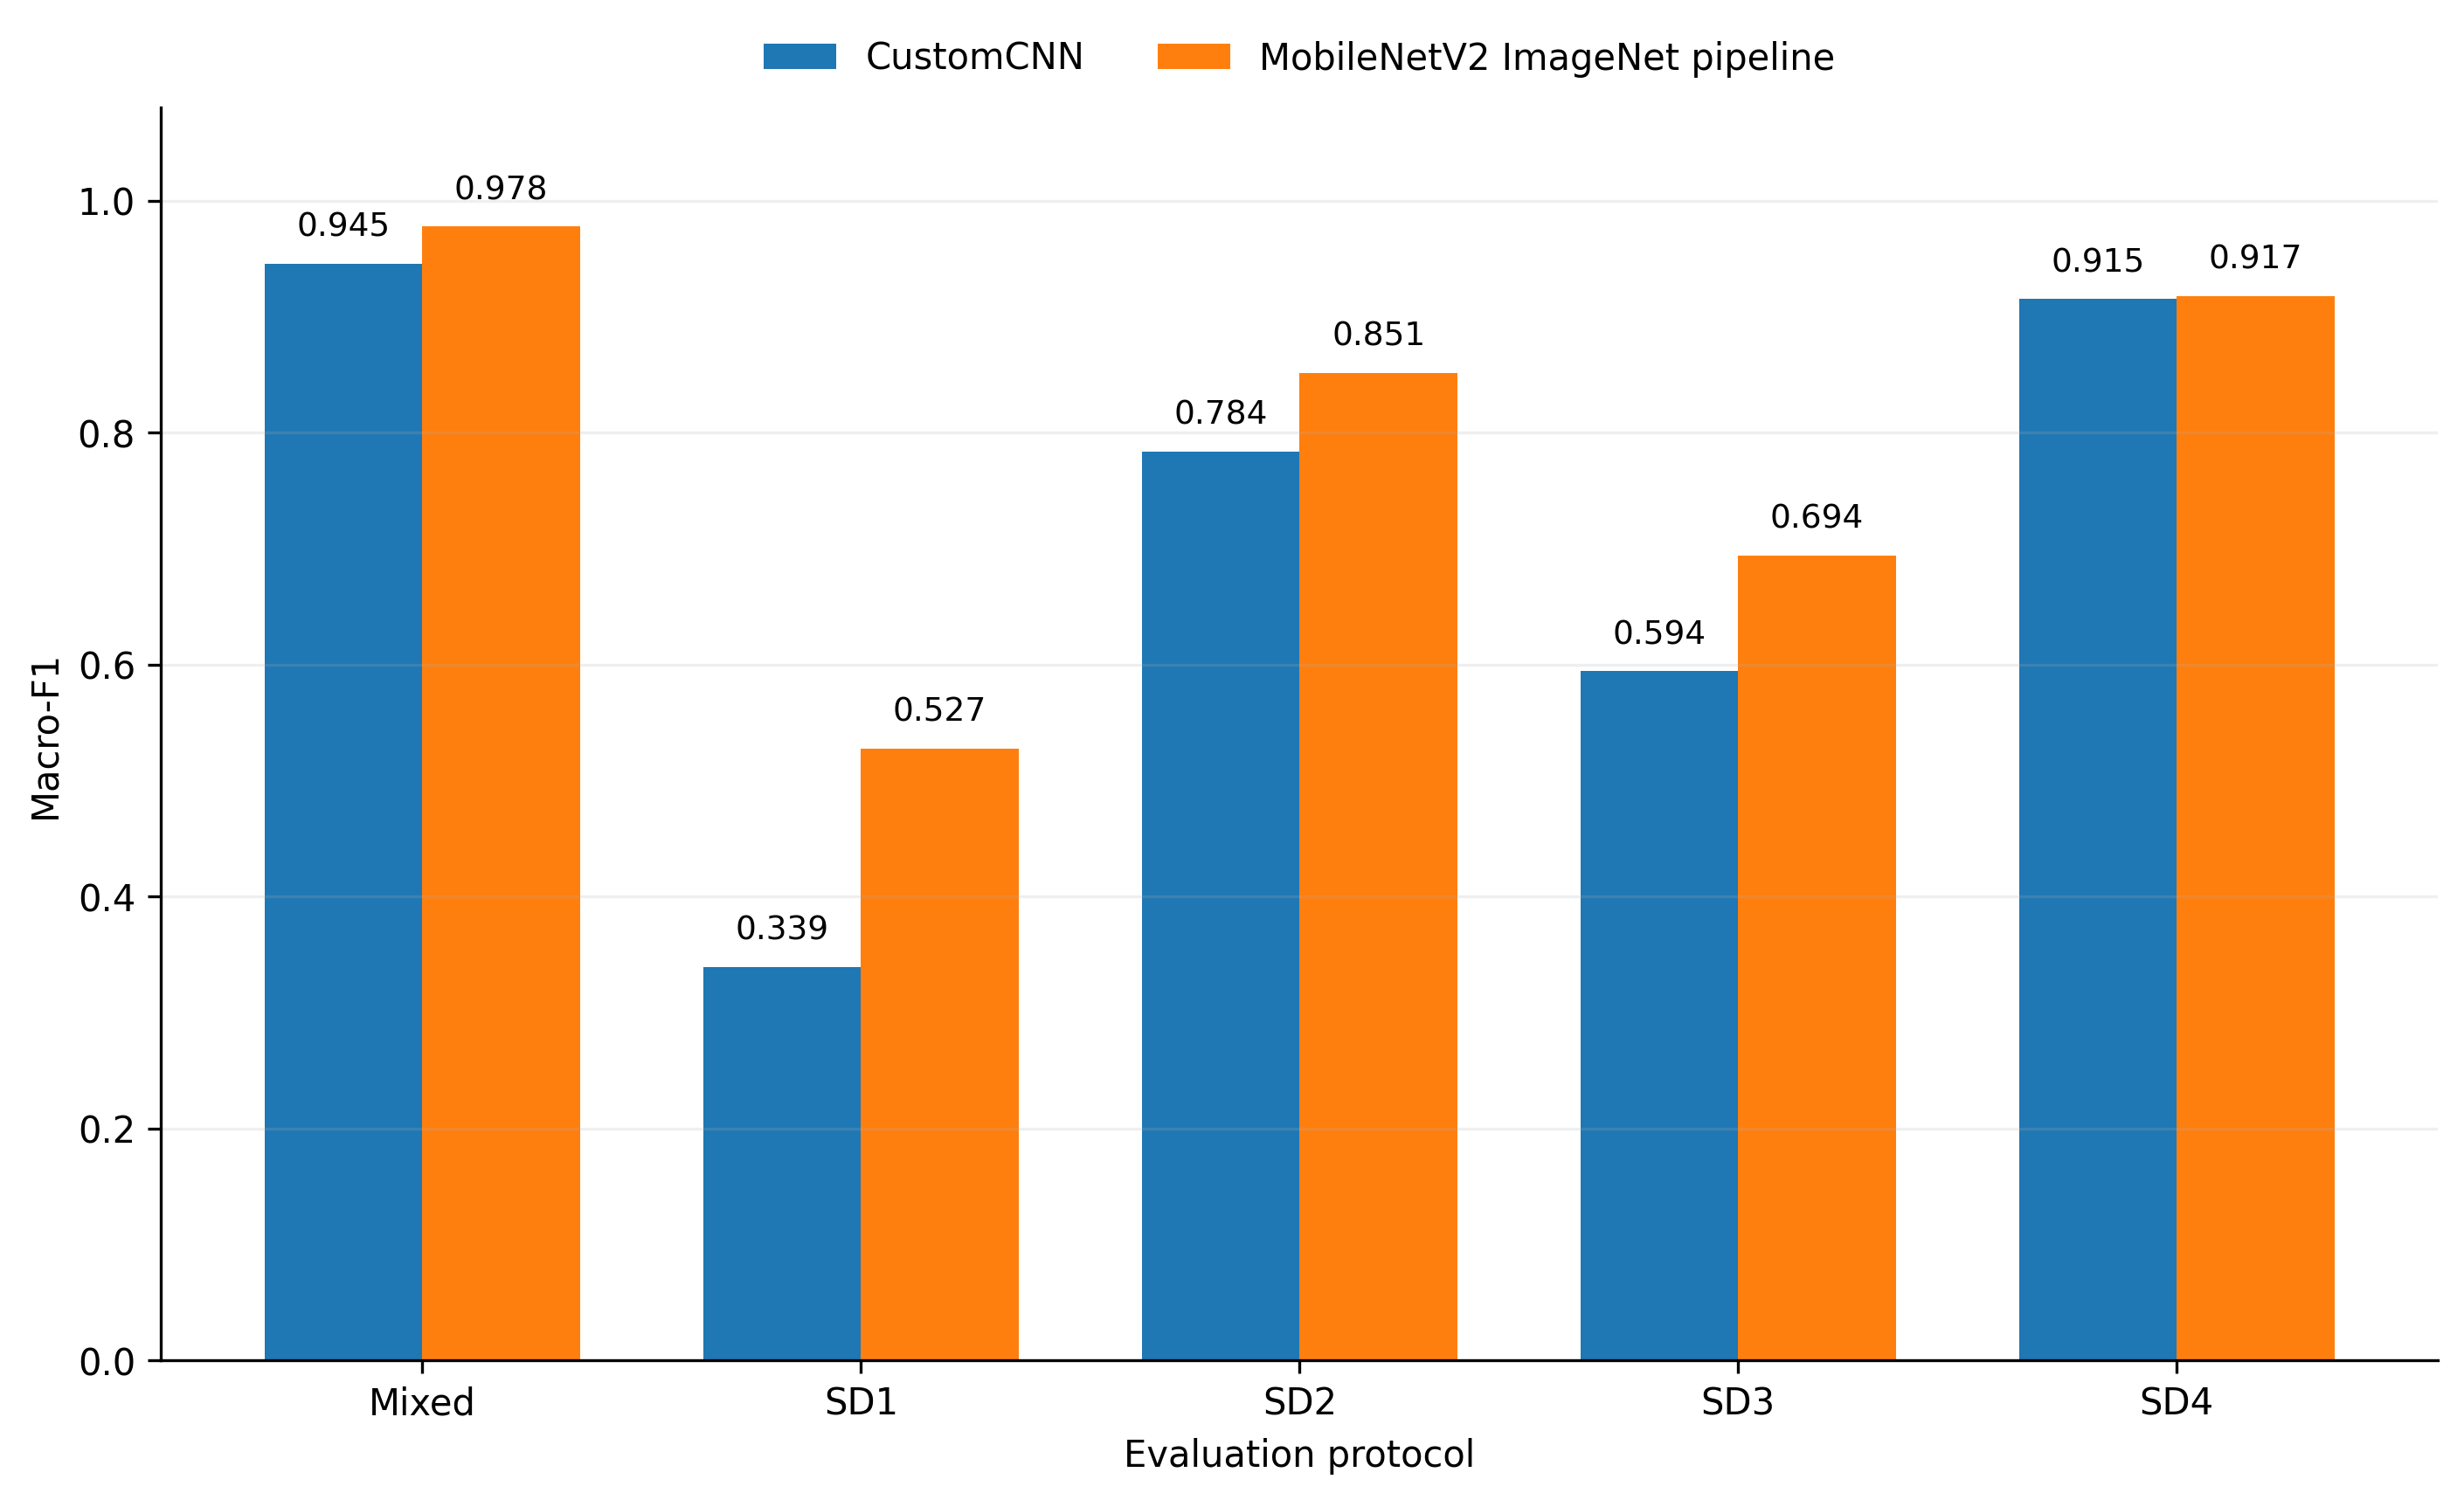
\includegraphics[width=0.84\textwidth]
{Fig_Mixed_vs_Source_Disjoint_MacroF1.png}
\caption{
Macro-F1 under mixed and source-disjoint evaluation.
Both pipelines achieve strong mixed-split performance but deteriorate
on unseen sources, particularly SD1. MobileNetV2 decreases from
0.9775 under mixed evaluation to 0.5274 on SD1, corresponding to a
45.0-percentage-point drop.
}
\label{fig:mixed_source}
\end{figure*}

Across SD1--SD4, CustomCNN achieves mean Macro-F1 0.6579 and
MobileNetV2 achieves 0.7476, an observed difference of 8.97 percentage
points. This should not be attributed solely to ImageNet pretraining
because architecture and training strategy also differ.

The substantial variation across the source-disjoint folds further
shows that apparent robustness depends strongly on which image sources
are withheld.

% ============================================================
% B. MULTI-SEED DG
% ============================================================

\subsection{Three-Seed Domain-Generalization Evaluation}


\begin{table}[t]
\centering
\caption{SD1 Three-Seed Replication}
\label{tab:sd1_multiseed}
\begin{tabular}{lcc}
\hline
Method & Seeds & Macro-F1 \\
\hline
ERM & 42, 123, 2026 & 0.4988$\pm$0.0259 \\
DG-AUG-V2 & 42, 123, 2026 & 0.4831$\pm$0.0443 \\
RSC & 42, 123, 2026 & 0.4883$\pm$0.0329 \\
\hline
\end{tabular}
\end{table}


ERM obtains $0.4988\pm0.0259$, DG-AUG-V2 obtains
$0.4831\pm0.0443$, and RSC obtains $0.4883\pm0.0329$.

Neither intervention consistently improves upon ERM. DG-AUG-V2 has a
lower mean and higher variability, whereas RSC is strongly
seed-sensitive. RSC improves over ERM for seed 2026 but performs worse
for seeds 42 and 123.

% ============================================================
% C. EXTERNAL FLOODNET
% ============================================================

\subsection{External FloodNet UAV Validation}


\begin{table*}[t]
\centering
\caption{Three-Seed Mean External FloodNet UAV Performance.
Supported Macro-F1 is computed over Flooded and Neither;
Desert predictions remain errors.}
\label{tab:floodnet_external}
\footnotesize
\setlength{\tabcolsep}{3.5pt}
\begin{tabular}{lccccccc}
\hline
Method & Acc. & Supp. F1 & AUROC & AUPRC &
Flood R. & Neither R. & False-Flood \\
\hline
ERM & 0.3886 & 0.3753$\pm$0.0468 & 0.7820 & 0.6305 & 0.9542 & 0.3055 & 0.6907 \\
DG-AUG-V2 & 0.3886 & 0.3729$\pm$0.0824 & 0.7730 & 0.6392 & 0.9477 & 0.3064 & 0.6907 \\
RSC & 0.3735 & 0.3619$\pm$0.0764 & 0.7848 & 0.6300 & 0.9804 & 0.2843 & 0.7109 \\
\hline
\end{tabular}
\end{table*}


ERM obtains supported-class Macro-F1
$0.3753\pm0.0468$. DG-AUG-V2 and RSC obtain
$0.3729\pm0.0824$ and $0.3619\pm0.0764$, respectively.

For ERM, mean Flooded recall is 0.9542 and mean Neither recall is
0.3055.

Among 347 external true-Neither scenes:

\begin{itemize}
    \item 178 (51.3\%) are predicted Flooded by all nine models,
    \item 56 (16.1\%) are predicted Neither by all nine models,
    \item 113 (32.6\%) show disagreement.
\end{itemize}

The agreement across methods and seeds indicates that this external
error is systematic rather than specific to a single model run.

% ============================================================
% COMBINE FORMER FIGURES 2 + 3
% ============================================================

\begin{figure*}[!t]
\centering

\begin{minipage}[t]{0.485\textwidth}
    \centering
    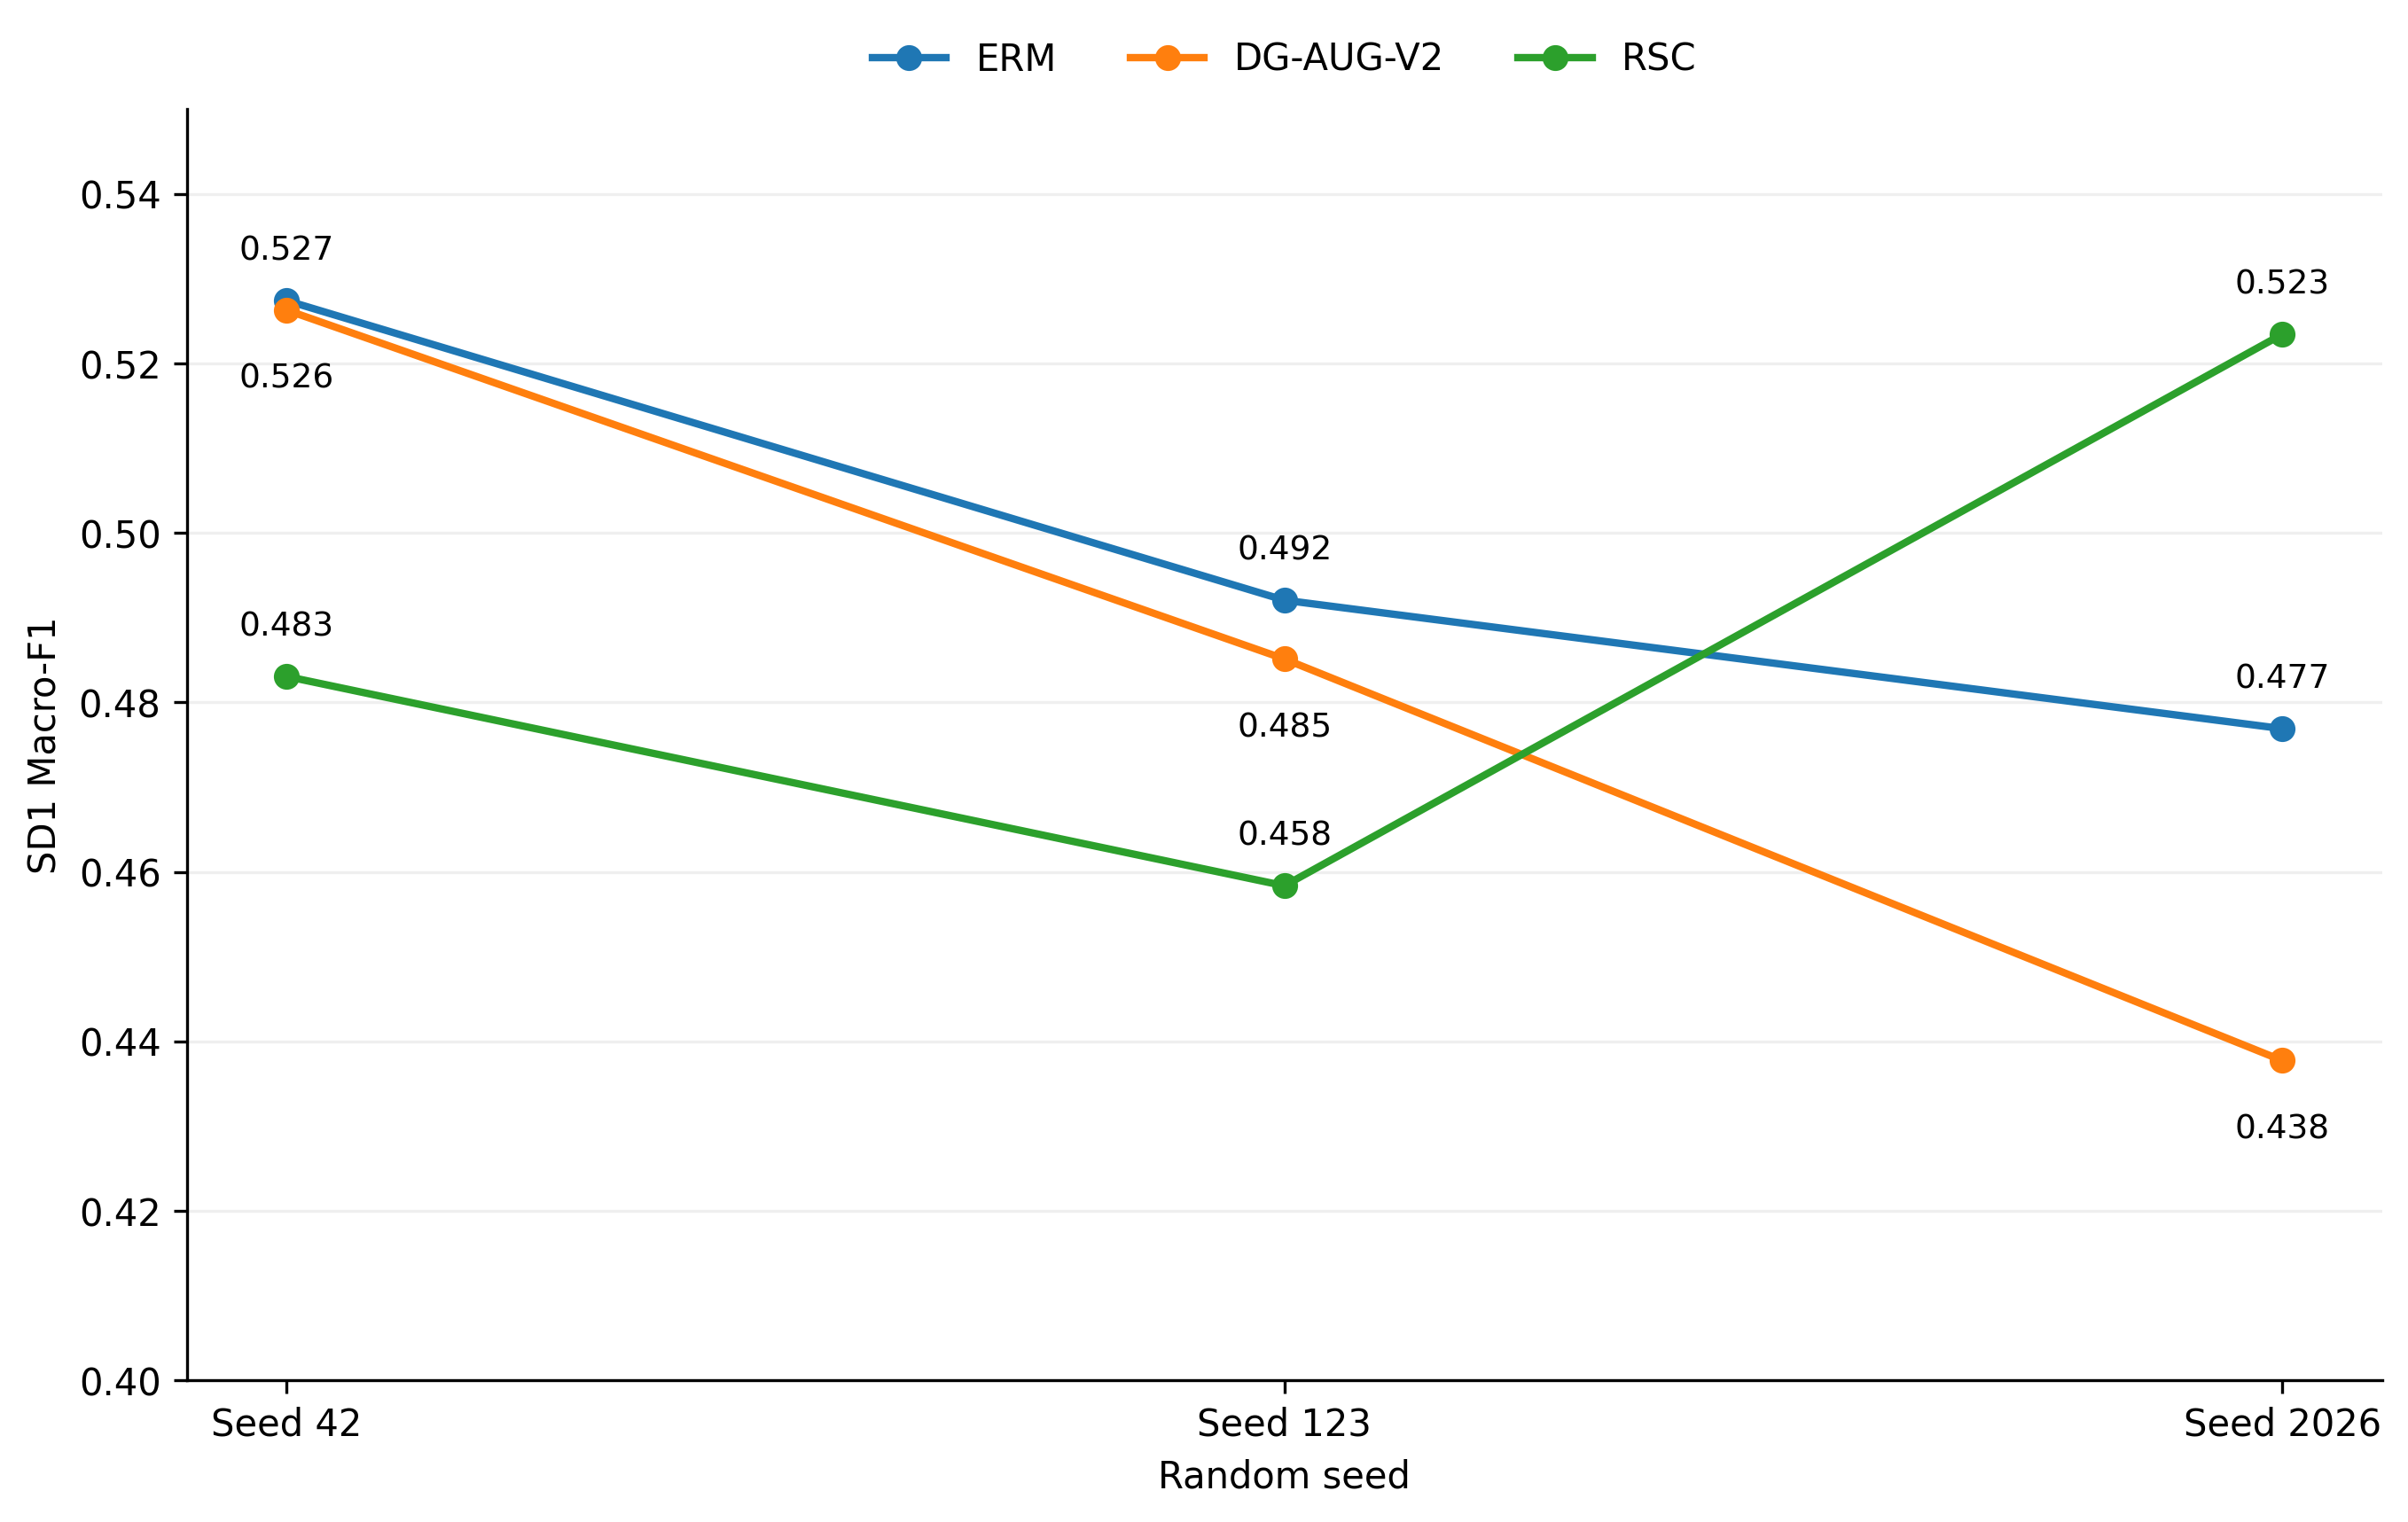
\includegraphics[width=\linewidth]
    {Fig_SD1_ThreeSeed_Method_Comparison.png}

    \vspace{-1mm}
    \textbf{(a)}
\end{minipage}
\hfill
\begin{minipage}[t]{0.485\textwidth}
    \centering
    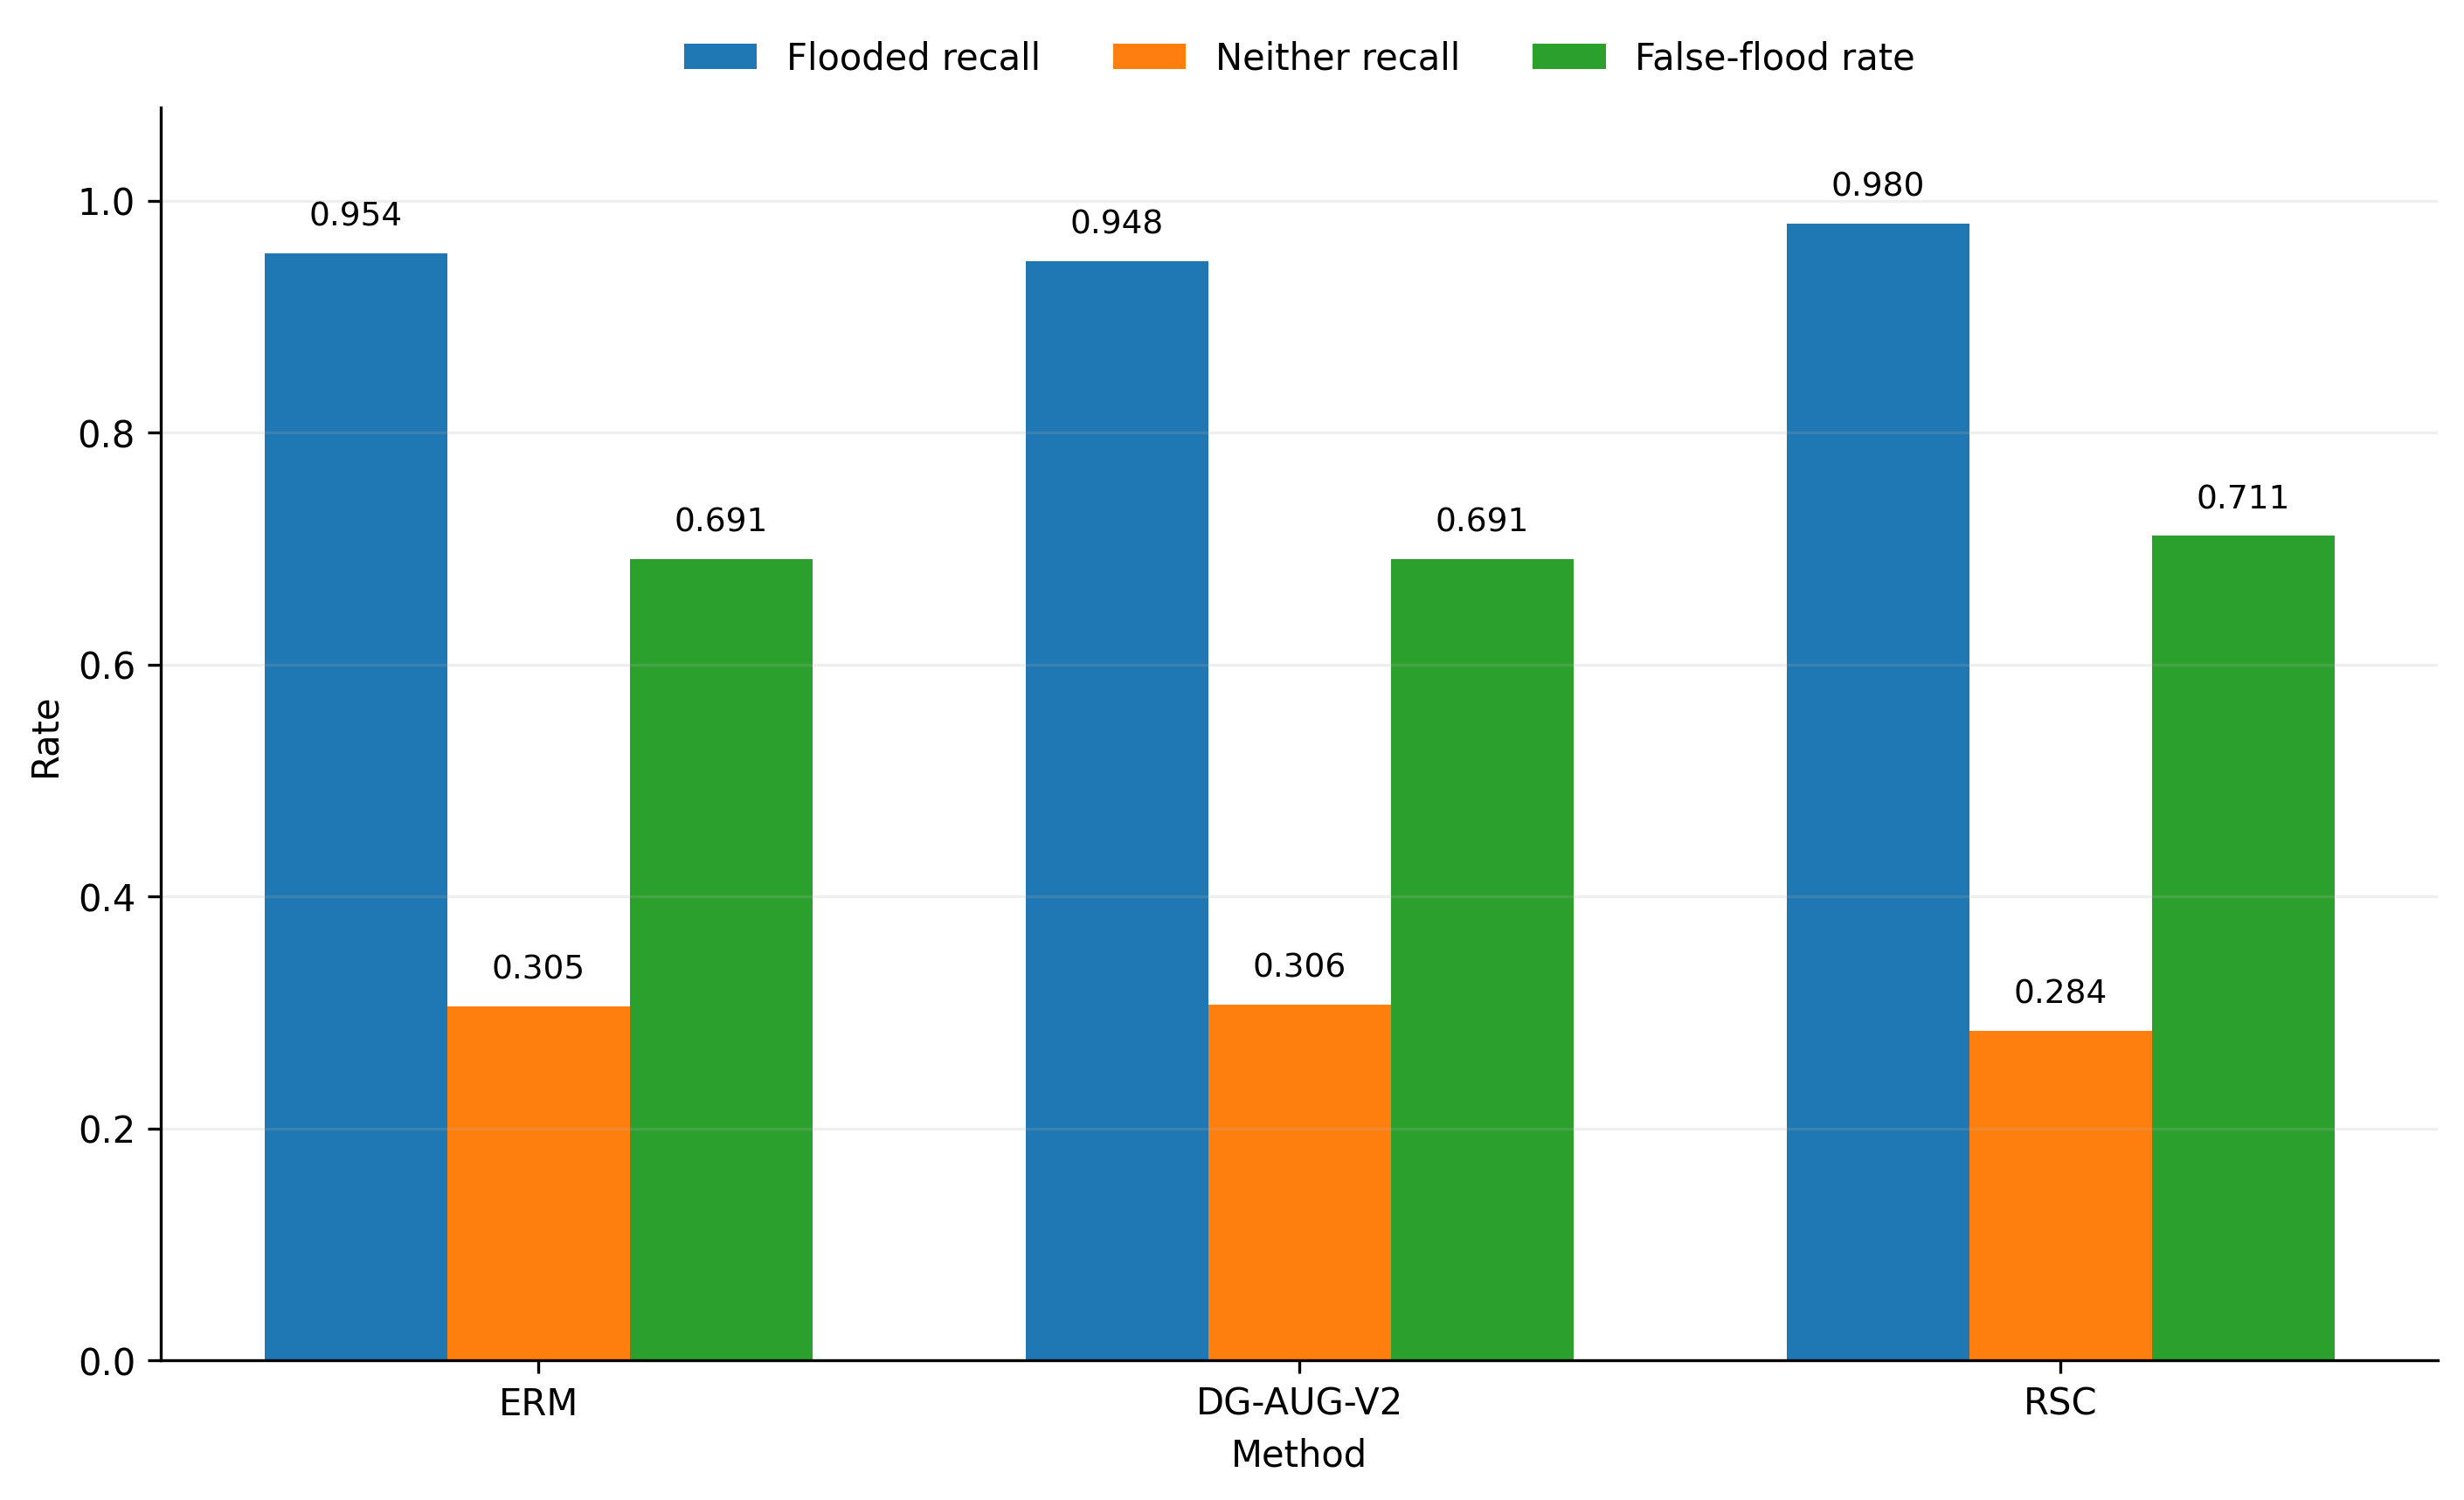
\includegraphics[width=\linewidth]
    {Fig_FloodNet_External_Asymmetric_Failure.png}

    \vspace{-1mm}
    \textbf{(b)}
\end{minipage}

\caption{
Robustness evaluation beyond the mixed split.
(a) SD1 Macro-F1 across seeds 42, 123, and 2026. RSC underperforms
ERM on two seeds but exceeds it on seed 2026, illustrating the danger
of drawing conclusions from a single favorable run.
(b) External FloodNet UAV evaluation. All three methods retain high
Flooded recall but exhibit low Neither recall and high false-flood
rates.
}
\label{fig:robustness_pair}
\end{figure*}

% ============================================================
% D. GRAD-CAM
% ============================================================

\subsection{Grad-CAM Analysis}

\begin{figure*}[!t]
\centering
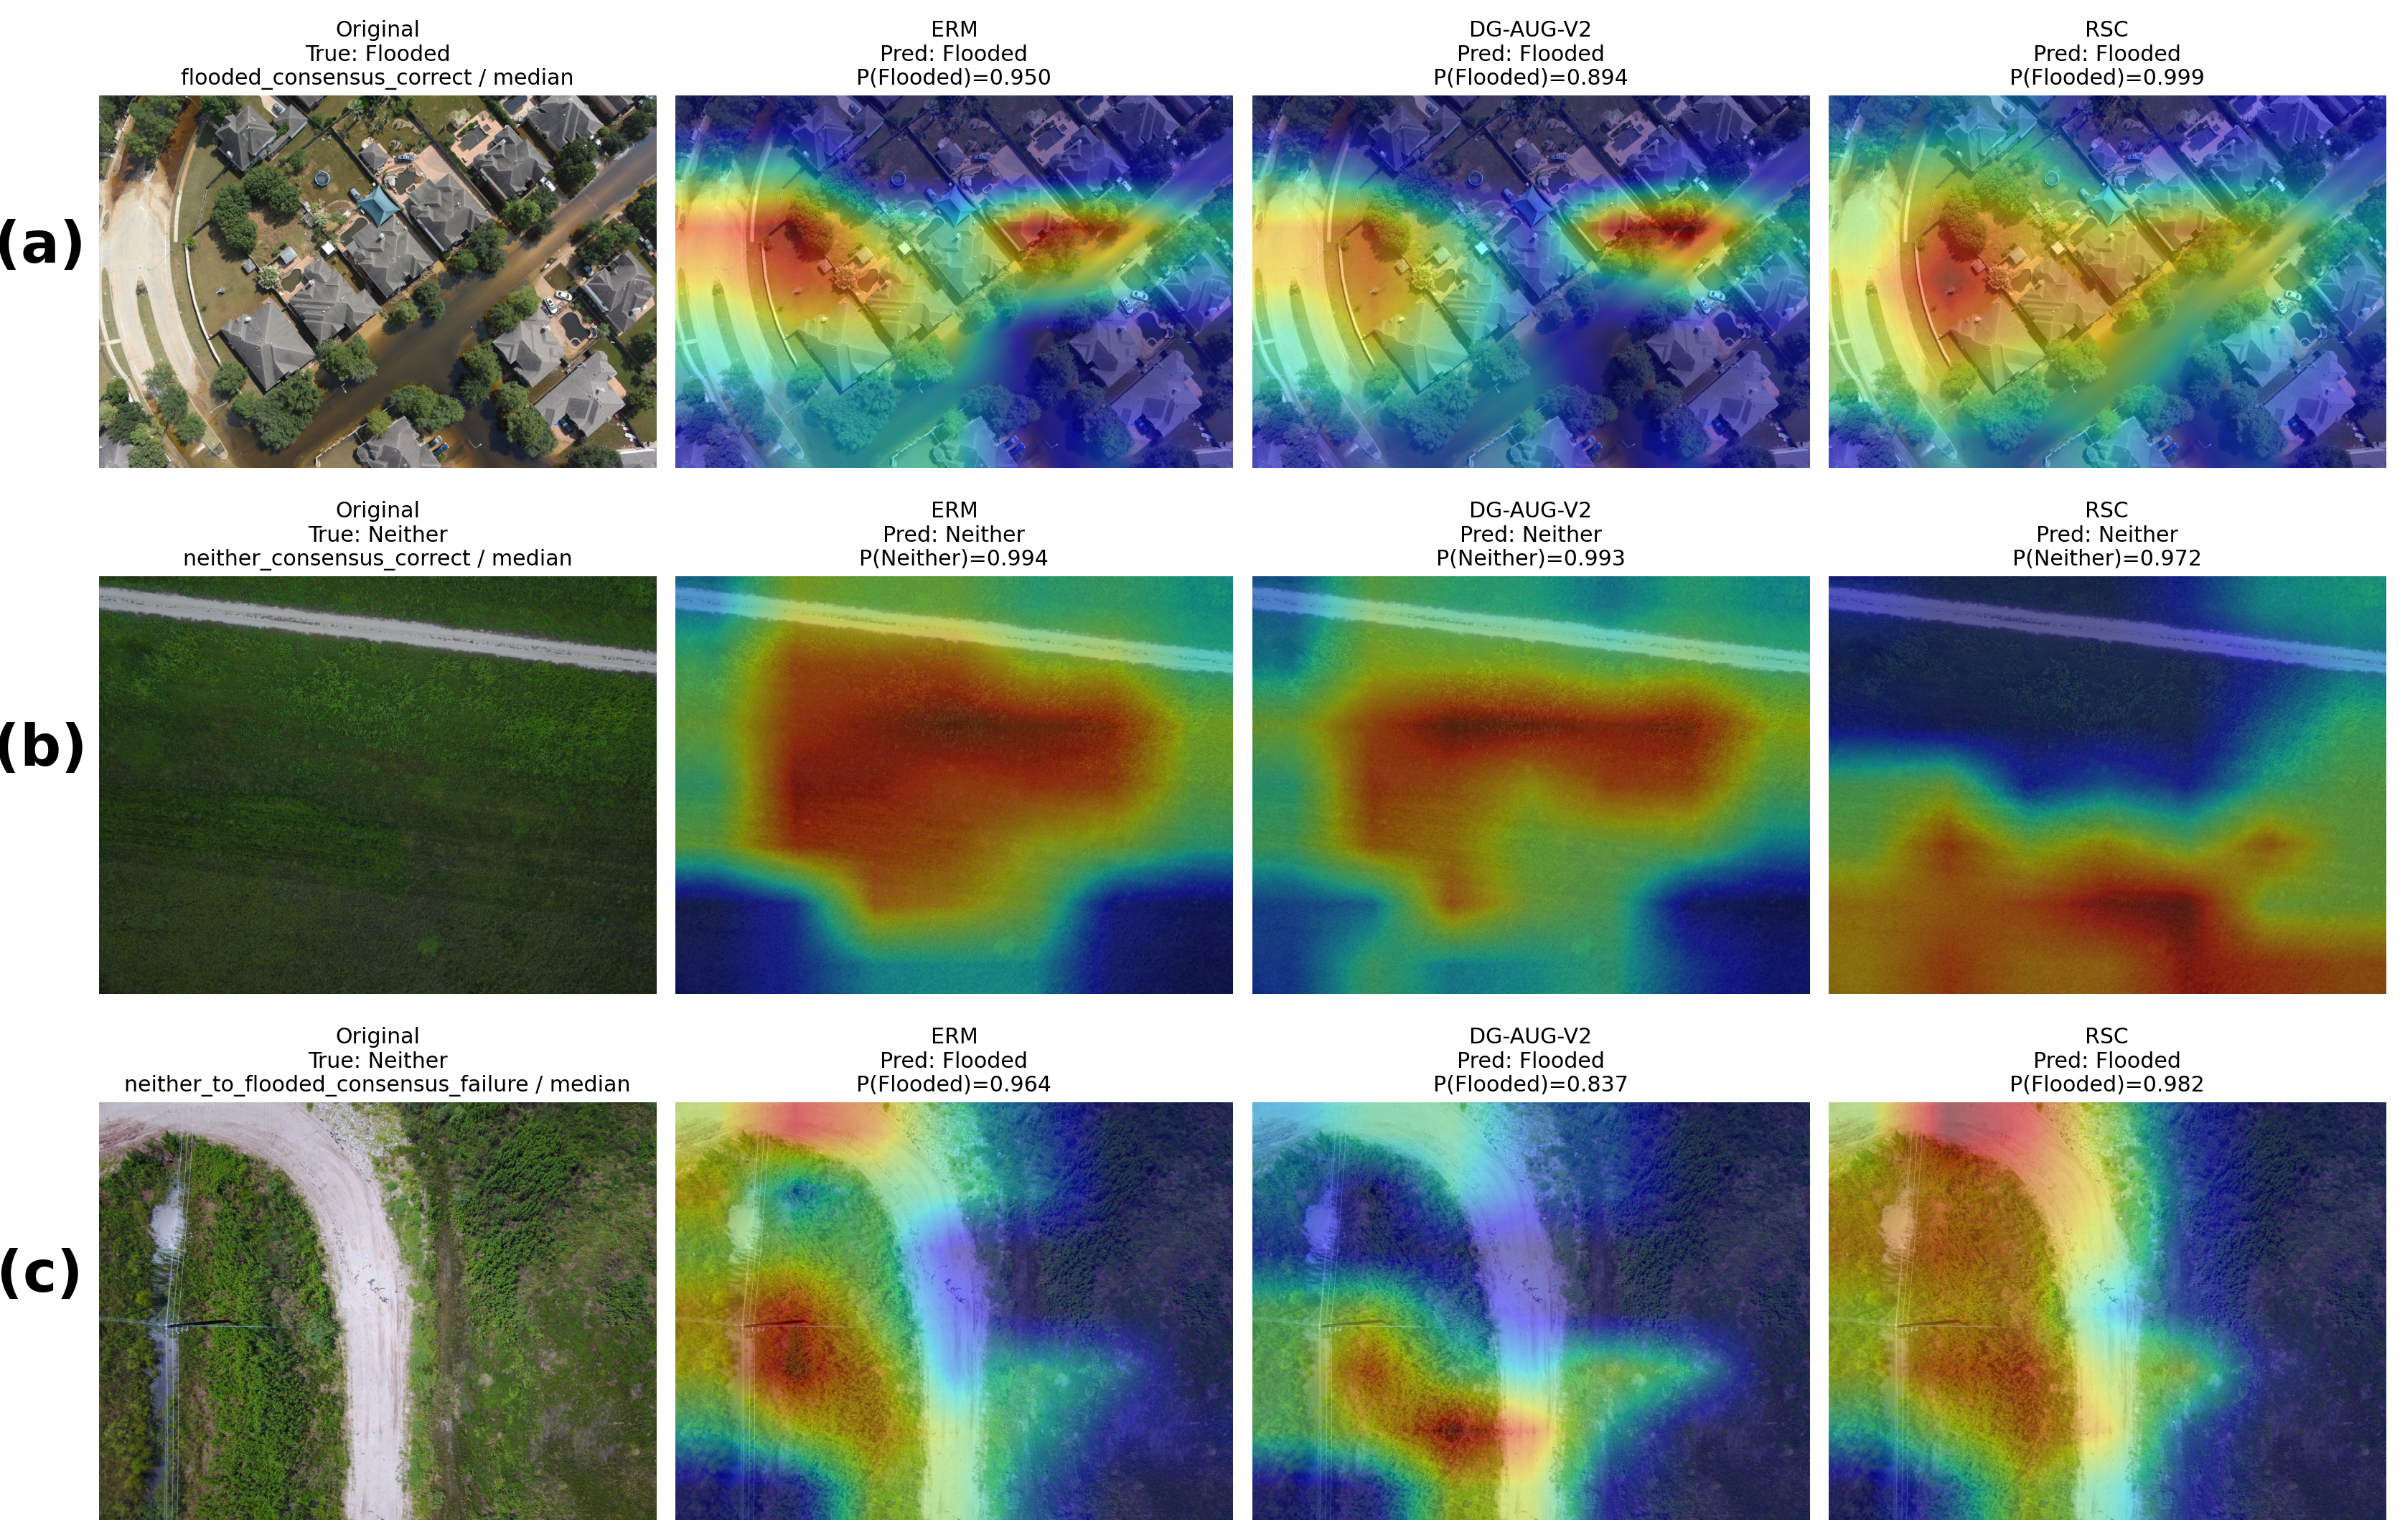
\includegraphics[width=0.92\textwidth]
{Fig_GradCAM_Representative_Median_Cases.png}
\caption{
Representative Grad-CAM visualizations from the frozen
median-confidence cohort.
(a) Consensus-correct Flooded scene,
(b) consensus-correct Neither scene, and
(c) consensus Neither-to-Flooded failure.
Columns show the original image and Grad-CAM maps from ERM,
DG-AUG-V2, and RSC.
}
\label{fig:gradcam}
\end{figure*}

Correct Neither scenes frequently emphasize homogeneous vegetation
and land texture. Several false-flood cases instead emphasize
water-like regions, roads, boundaries, and adjacent infrastructure.

ERM and DG-AUG-V2 often produce similar spatial activation patterns,
whereas RSC tends to produce broader or spatially shifted activation.

These maps are qualitative explanatory evidence and are not interpreted
as causal proof of the model's decision process.

% ============================================================
% E. SEGMENTATION SHORTCUT ANALYSIS
% ============================================================

\subsection{Segmentation-Based Failure Analysis}


\begin{table*}[t]
\centering
\caption{Post-Hoc Segmentation Composition of Consensus
False-Flood ($n=178$) and Consensus-Correct Neither ($n=56$)
Scenes. Reported $p$-values are Holm-adjusted across all ten
segmentation classes. Road-flooded and Building-flooded pixels
were absent from both consensus groups.}
\label{tab:segmentation_shortcut}
\footnotesize
\setlength{\tabcolsep}{4pt}
\begin{tabular}{lrrrrrr}
\hline
Class &
Fail Pres. (\%) &
Corr. Pres. (\%) &
Fail Area (\%) &
Corr. Area (\%) &
Fisher $p_{\mathrm{Holm}}$ &
MW $p_{\mathrm{Holm}}$ \\
\hline
Water & 51.7 & 5.4 & 13.44 & 0.53 & 2.42e-10 & 9.27e-09 \\
Road-non-flooded & 73.0 & 14.3 & 8.84 & 0.58 & 3.95e-14 & 3.85e-13 \\
Grass & 93.8 & 100.0 & 51.88 & 85.25 & 0.2823 & 2.02e-16 \\
Tree & 89.9 & 58.9 & 18.78 & 13.22 & 4.67e-06 & 5.18e-04 \\
\hline
\end{tabular}
\end{table*}


Water is present in 51.7\% of consensus false-flood scenes but only
5.4\% of consensus-correct Neither scenes. After Holm correction:

\[
p_{\mathrm{Holm}}=2.42\times10^{-10}.
\]

Non-flooded roads are present in 73.0\% of failures and 14.3\% of
correct scenes:

\[
p_{\mathrm{Holm}}=3.95\times10^{-14}.
\]

Grass presence itself is not significantly different after Holm
correction. However, mean Grass coverage is 51.88\% in failures and
85.25\% in correct scenes:

\[
p_{\mathrm{Holm}}=2.02\times10^{-16}.
\]

Road-flooded and Building-flooded pixels are absent from both
consensus groups.

% ============================================================
% COMBINE FORMER SEGMENTATION FIGURES 5 + 6
% ============================================================

\begin{figure*}[!t]
\centering

\begin{minipage}[t]{0.32\textwidth}
    \centering
    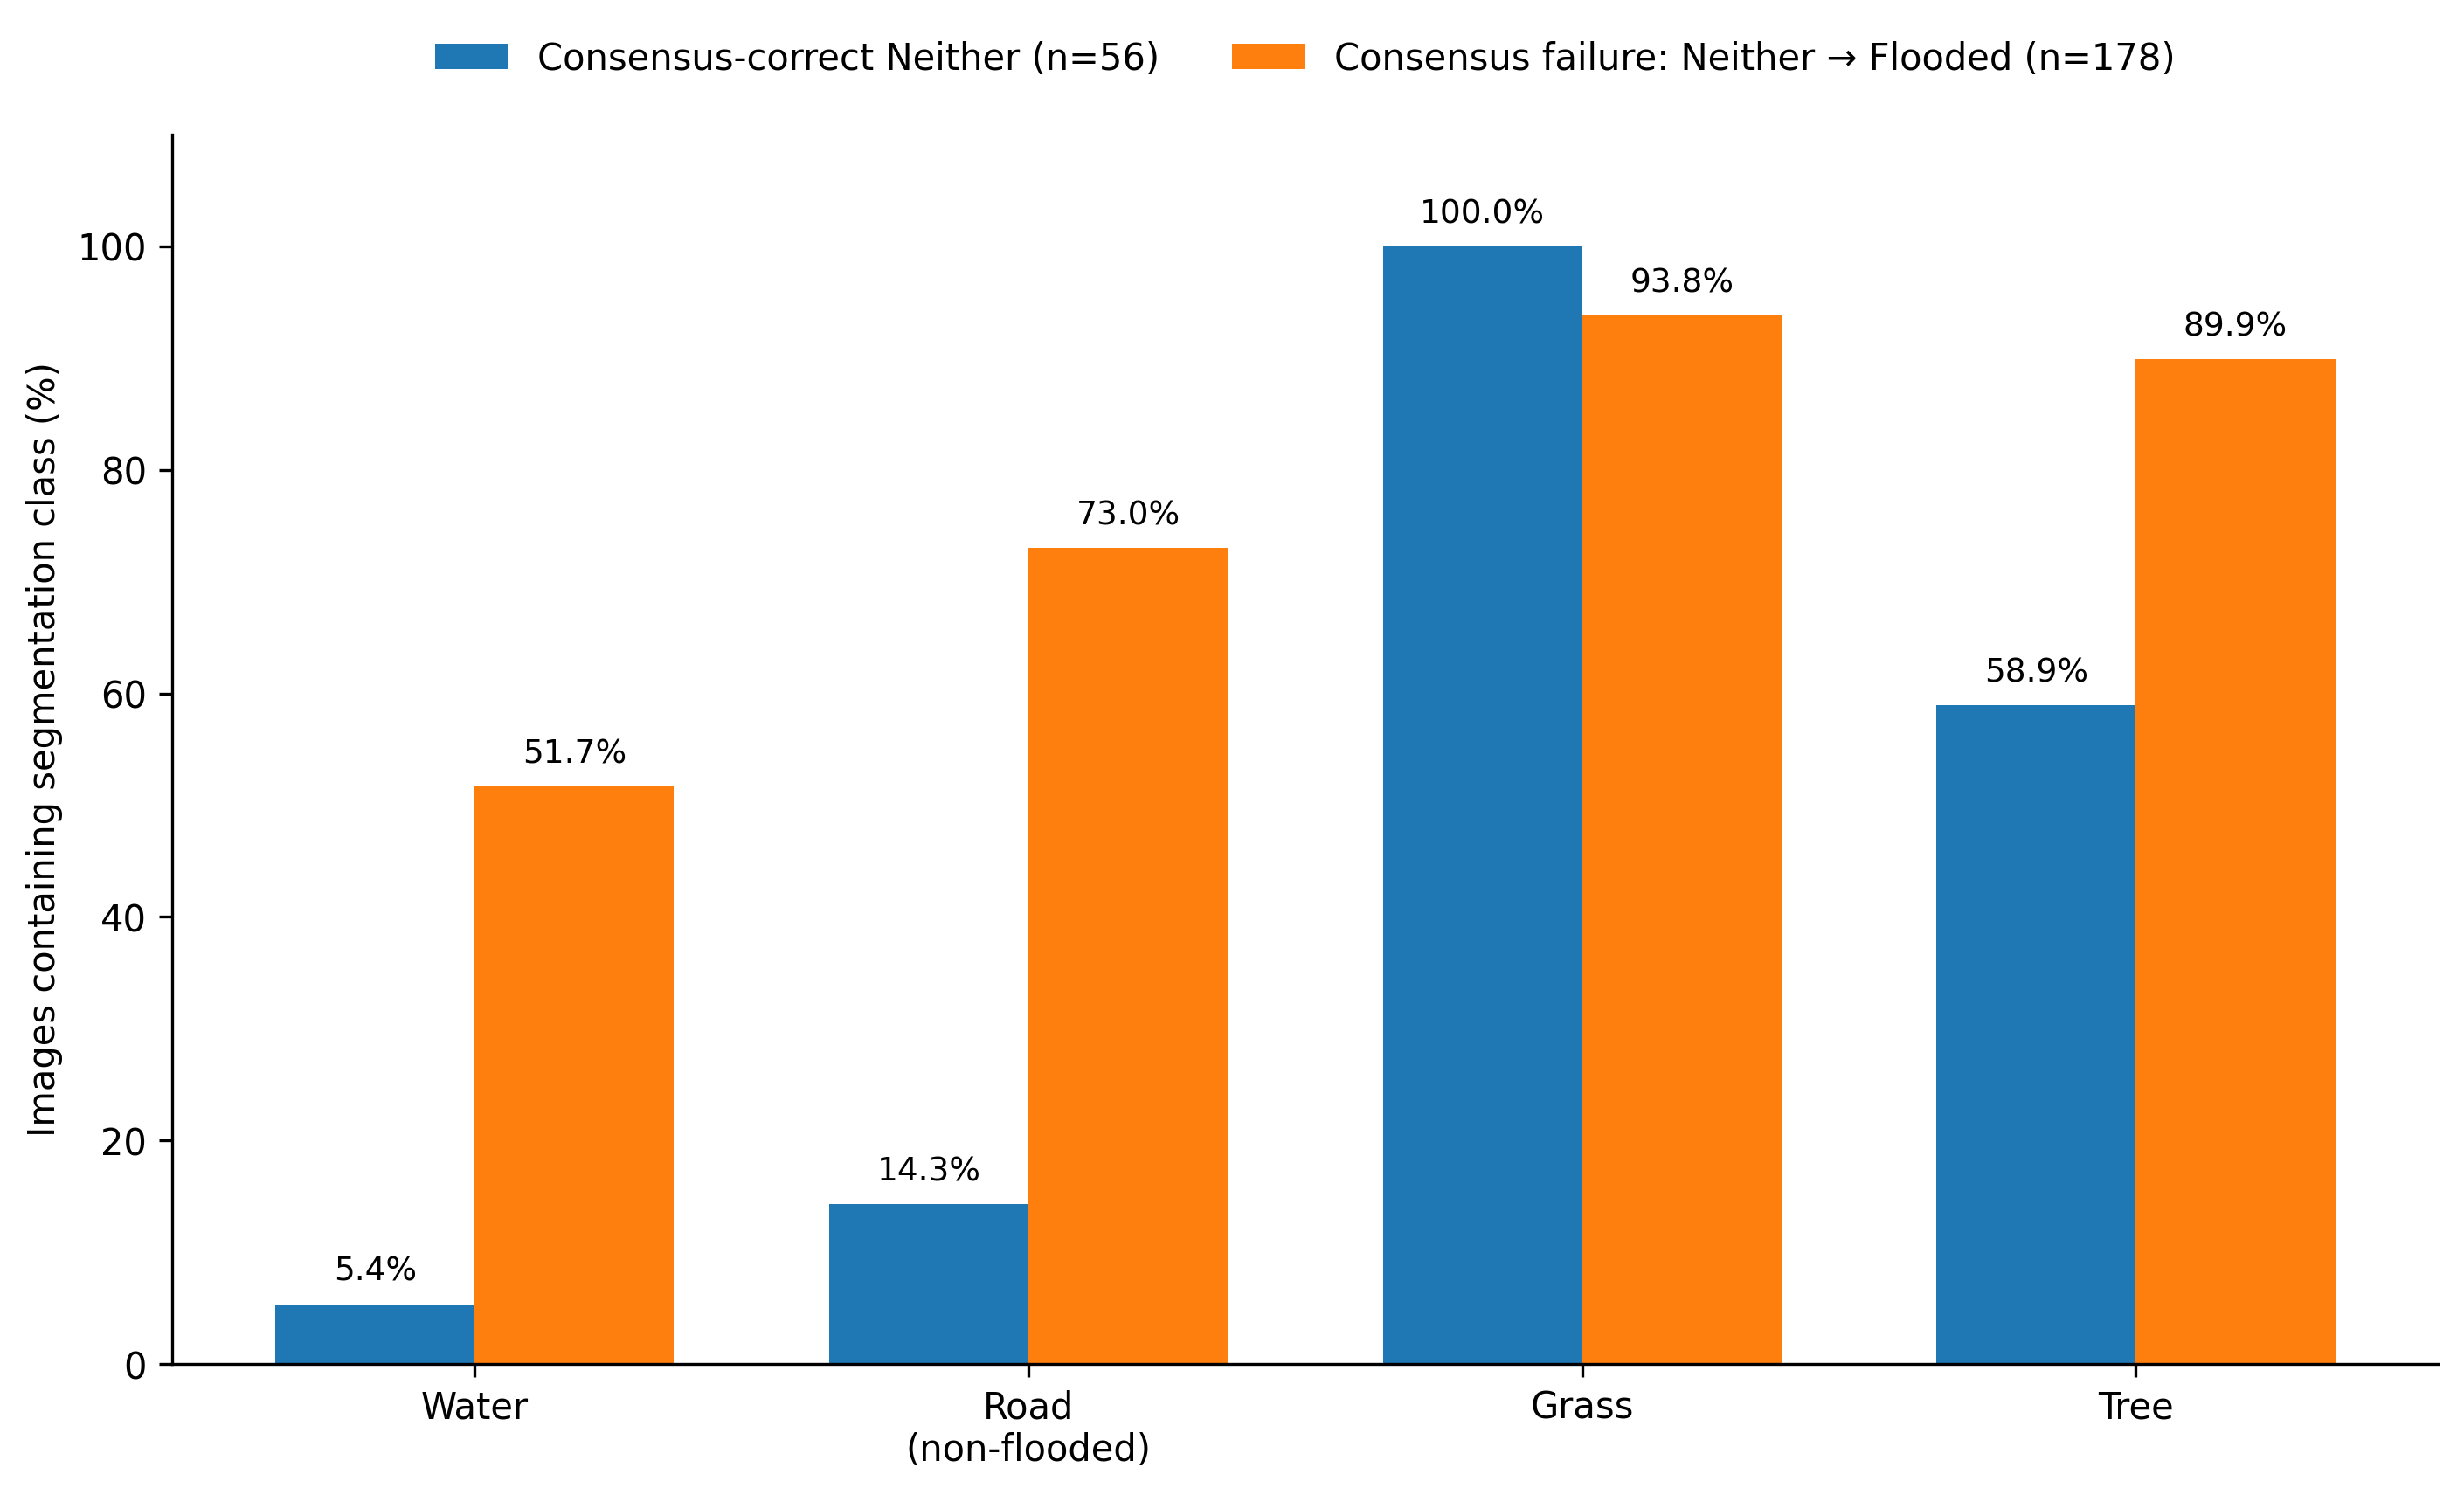
\includegraphics[width=\linewidth]
    {Fig_segmentation_class_presence_rates.png}

    \vspace{-1mm}
    \textbf{(a)}
\end{minipage}
\hfill
\begin{minipage}[t]{0.32\textwidth}
    \centering
    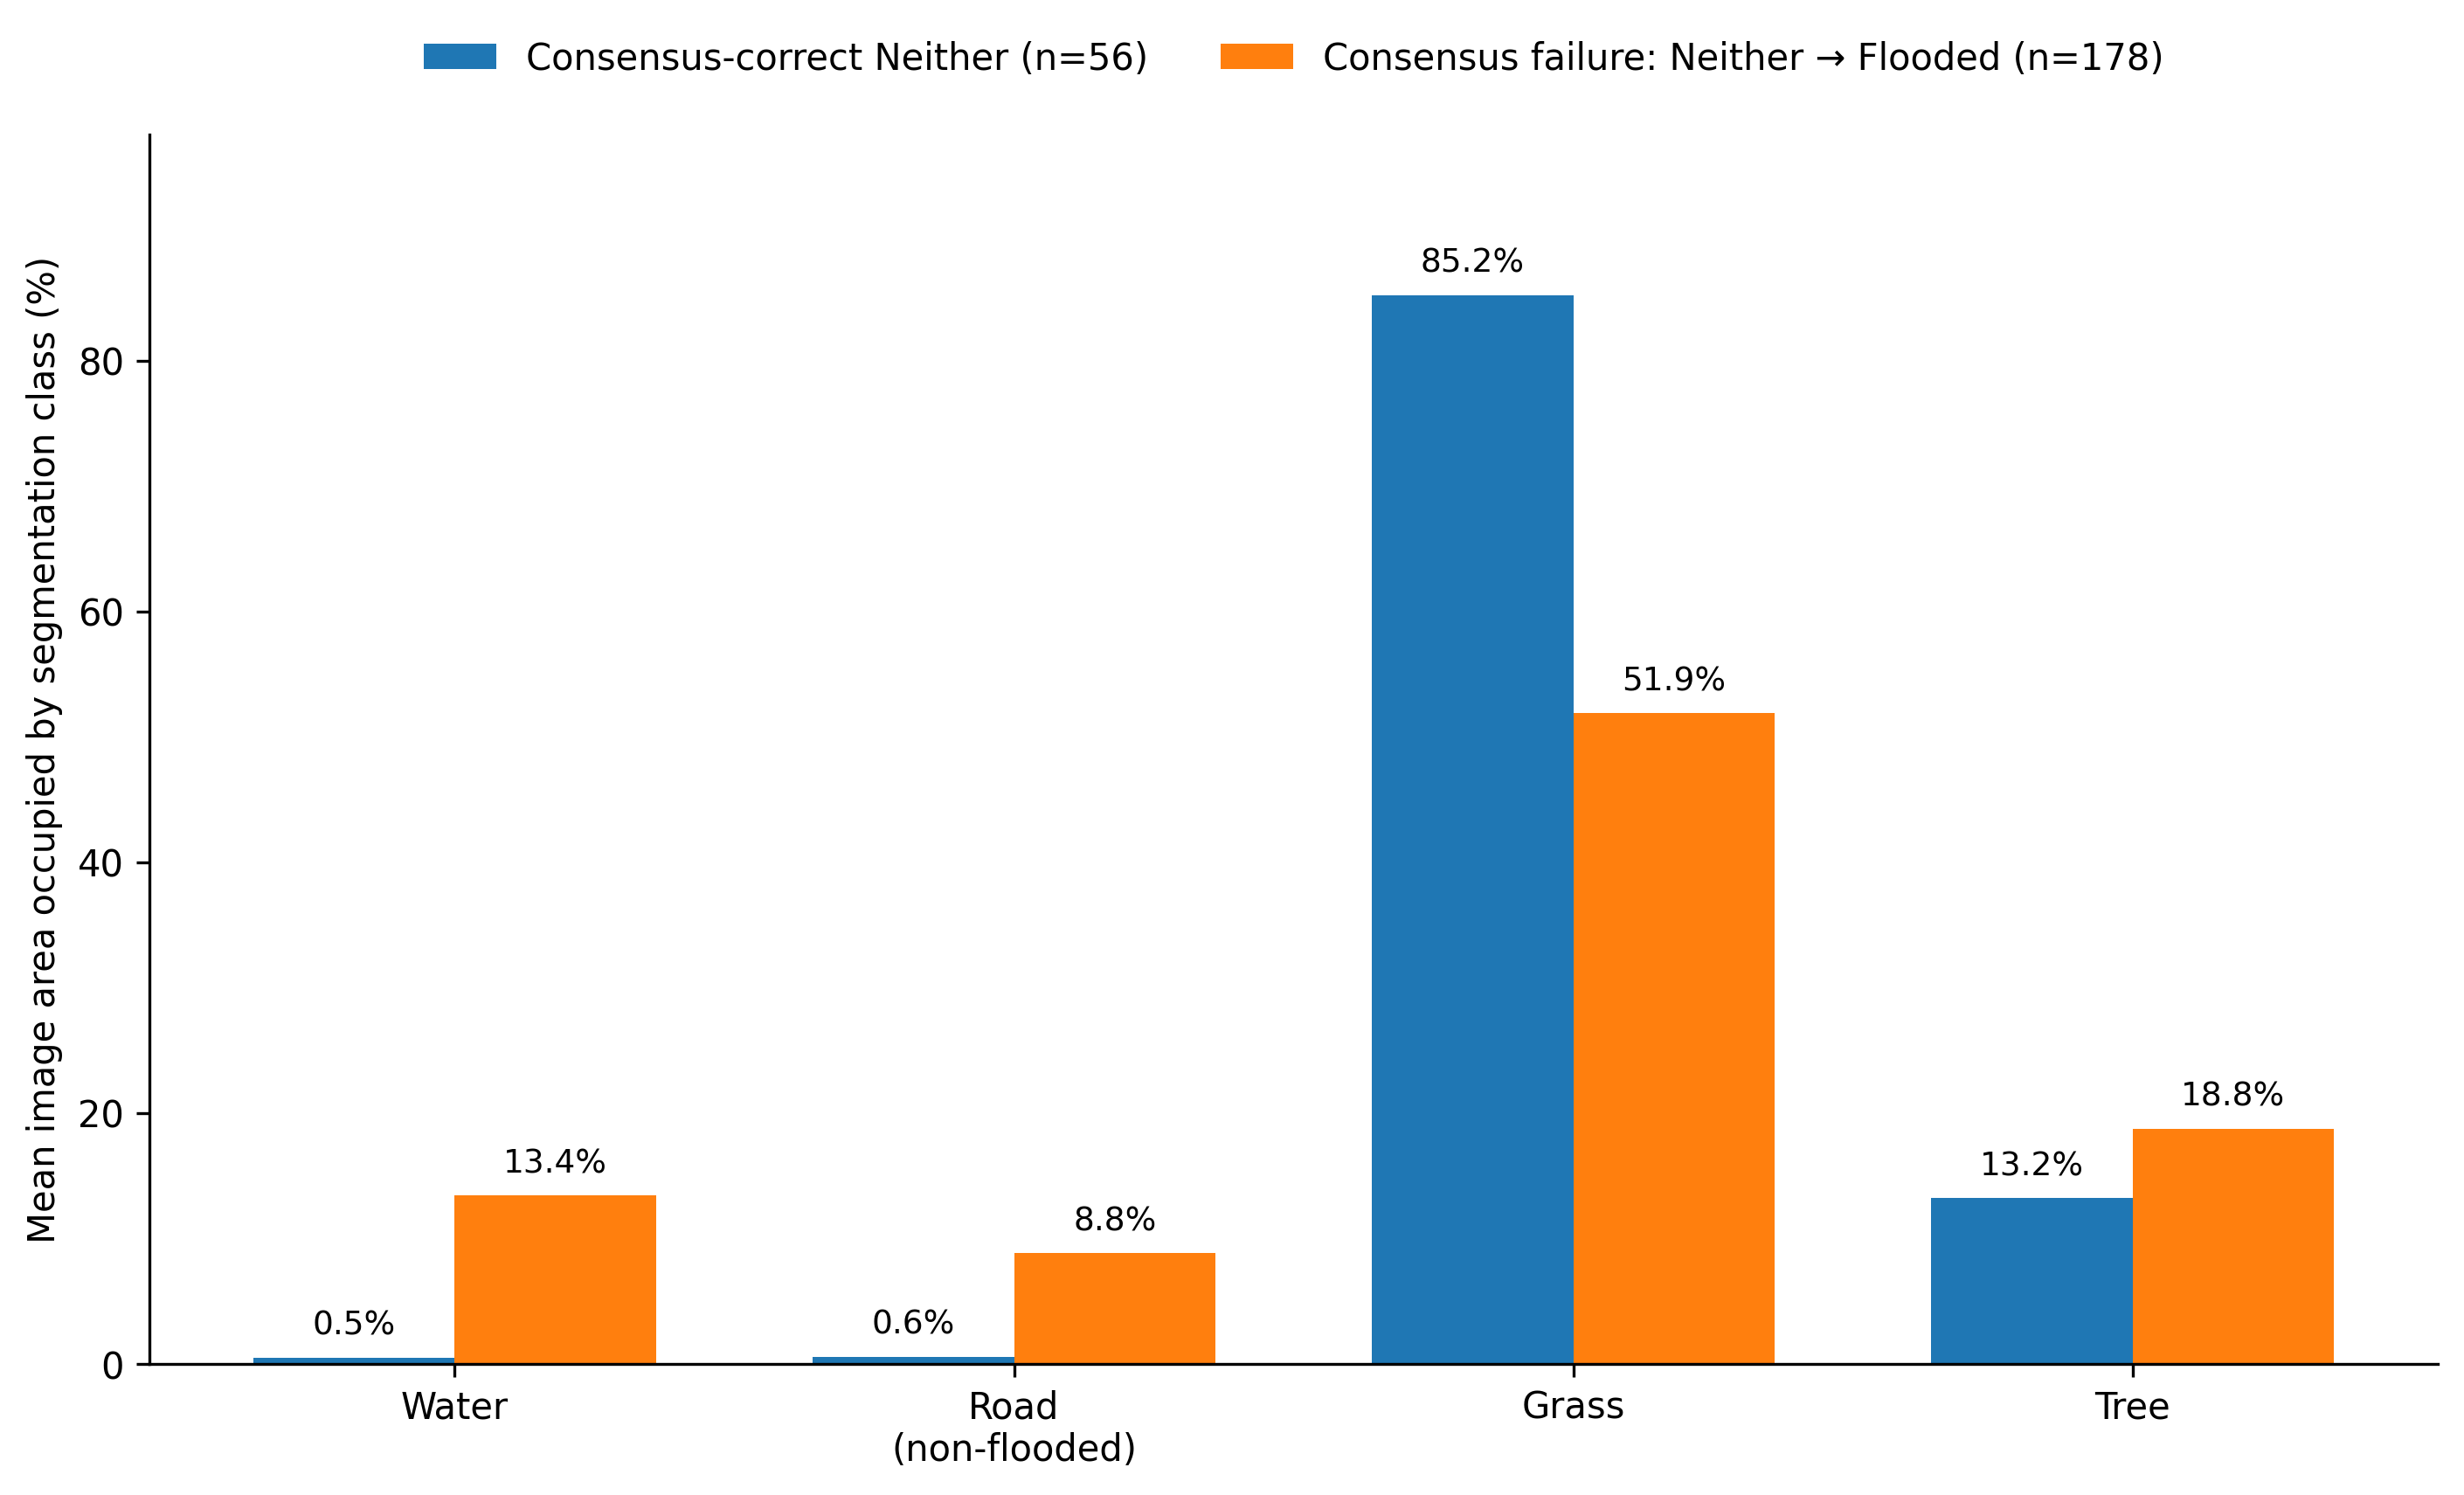
\includegraphics[width=\linewidth]
    {Fig_segmentation_mean_pixel_coverage.png}

    \vspace{-1mm}
    \textbf{(b)}
\end{minipage}
\hfill
\begin{minipage}[t]{0.32\textwidth}
    \centering
    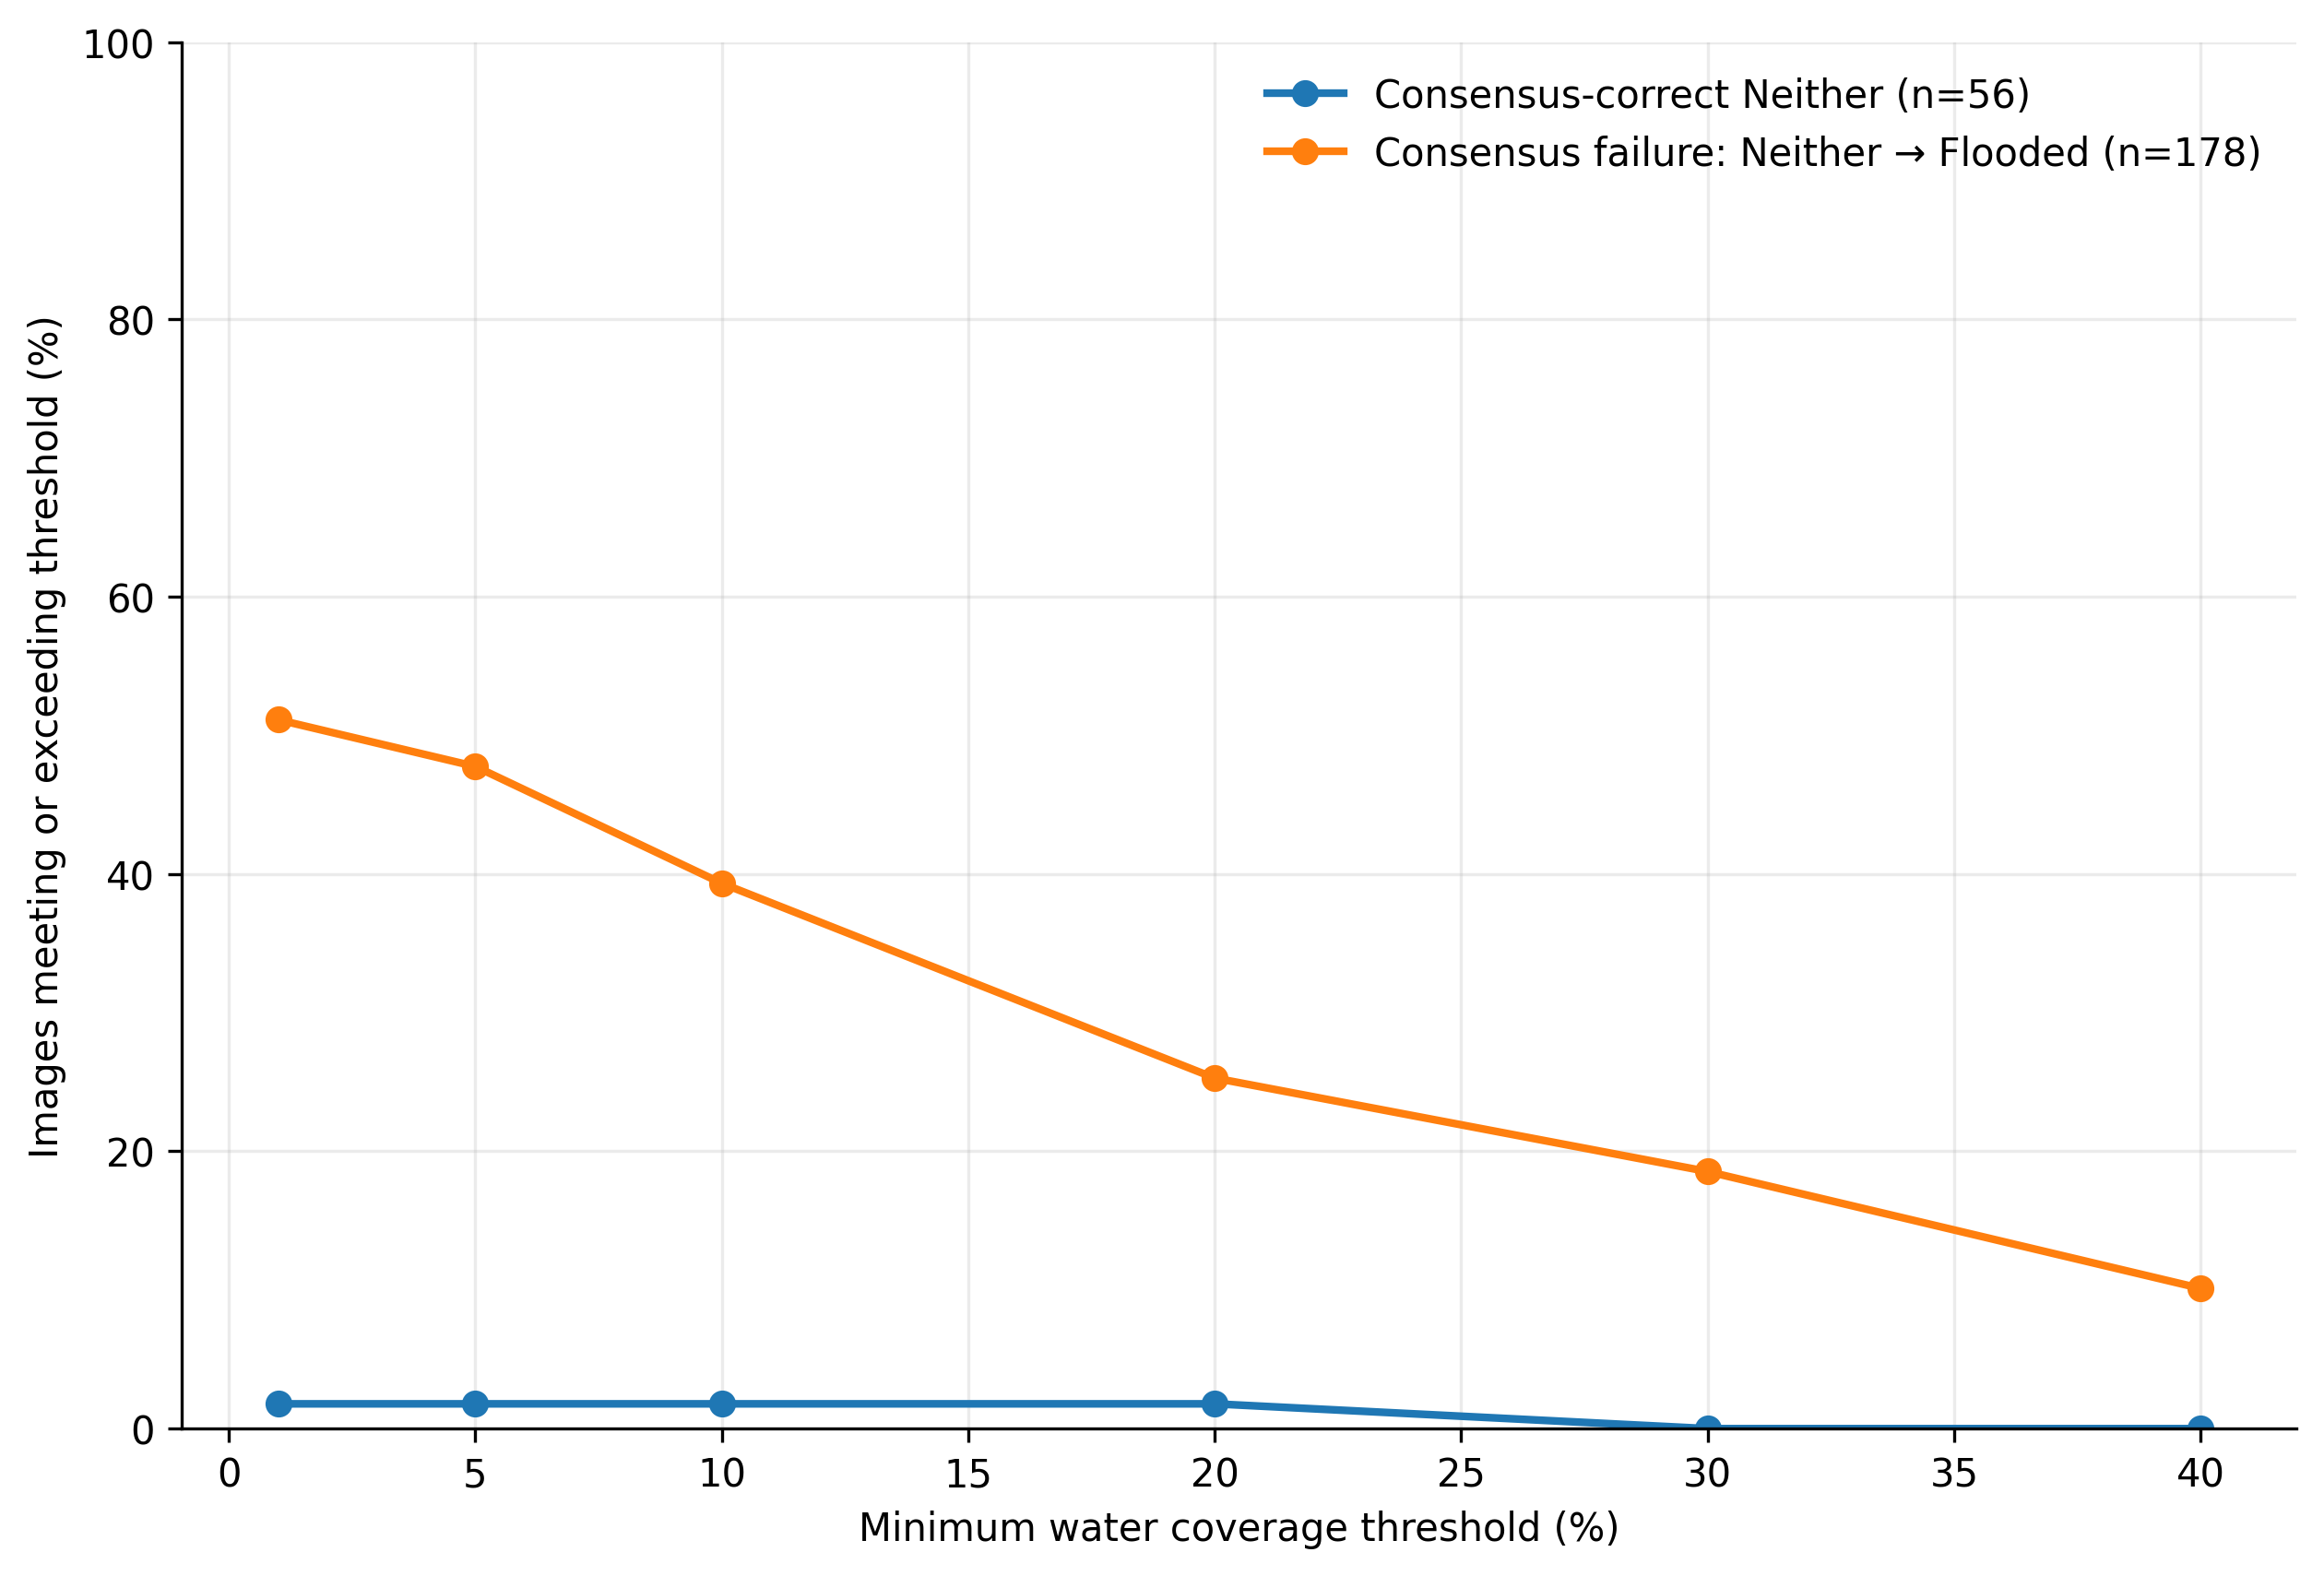
\includegraphics[width=\linewidth]
    {Fig_water_coverage_threshold_curve.png}

    \vspace{-1mm}
    \textbf{(c)}
\end{minipage}

\caption{
Post-hoc FloodNet segmentation analysis.
(a) Segmentation-class presence rates.
(b) Mean image area occupied by each segmentation class.
(c) Fraction of consensus-failure and consensus-correct Neither scenes
meeting increasingly strict Water-coverage thresholds.
Consensus false-flood scenes contain substantially more ordinary Water
and non-flooded Road context and are less strongly grass-dominated.
}
\label{fig:segmentation_triptych}
\end{figure*}

Taken together with the Grad-CAM observations, the segmentation
analysis is consistent with reliance on flood-associated contextual
cues, including ordinary water, non-flooded roads, and heterogeneous
terrain, rather than a complete semantic distinction between ordinary
water and true inundation.

Because the segmentation hypothesis was developed after observing the
external failure pattern, these results establish association rather
than causality.

% Ensure Results floats appear before Limitations.
\clearpage

\section{Limitations and Future Work}
\label{sec:limitations}

First, source identity, semantic class, and acquisition modality are
partially confounded, so the internal source-disjoint experiments do
not isolate a purely causal UAV-versus-satellite shift.

Second, FloodNet supports only Flooded and Non-Flooded ground truth,
although the original three-class model output is preserved.

Third, the segmentation shortcut analysis is post hoc and should be
interpreted as exploratory association rather than causal evidence.

Fourth, Grad-CAM provides spatial sensitivity information but does not
prove causal decision mechanisms.

Fifth, the CustomCNN and MobileNetV2 pipelines differ in architecture
and training strategy, so their performance difference cannot be
attributed solely to ImageNet pretraining.

Future work should evaluate additional recent external UAV and
satellite datasets, use acquisition-balanced datasets, investigate
segmentation-aware models, evaluate calibration, and perform causal
context interventions.

\section{Conclusion}
\label{sec:conclusion}

This study demonstrates that high mixed-split climate-scene
classification performance does not guarantee cross-source
robustness.

MobileNetV2 achieves a mixed Macro-F1 of 0.9775 but decreases to
0.5274 on SD1. Three-seed experiments show that DG-AUG-V2 and RSC do
not consistently outperform ERM.

External FloodNet validation independently reproduces a strong
Neither-to-Flooded failure. Among 347 true-Neither scenes, 178 are
classified as Flooded by all nine frozen models.

Grad-CAM and official FloodNet segmentation masks further show that
these failures are strongly associated with ordinary water,
non-flooded roads, and heterogeneous scene composition.

The results highlight the importance of source-aware evaluation,
multi-seed replication, independent external validation, and explicit
failure analysis when assessing deep-learning systems for
climate-related aerial imagery.


% Acknowledgment will be inserted after final author/disclosure review.



\bibliographystyle{IEEEtran}
\bibliography{references}

\end{document}
